\documentclass[12pt]{report}
\usepackage[utf8]{inputenc}

\title{SPATIAL ENHANCEMENT OF REMOTELY SENSED IMAGES USING CONVOLUTIONAL NEURAL NETWORKS}
\author{Palatucci Ugo}
\date{July 2020}

\usepackage{graphicx}
\usepackage{url}
\usepackage{amsmath}
\usepackage[margin=1.5in]{geometry}
\usepackage{listings}
\usepackage{setspace}

\linespread{1.75}

\begin{document}

\newgeometry{margin=1.5in}

\begin{titlepage}
    \begin{center}
        \vspace*{1cm}
            
        \large
        \textbf{SPATIAL ENHANCEMENT OF REMOTELY SENSED IMAGES USING CONVOLUTIONAL NEURAL NETWORKS}
            
        \vspace{0.5cm}
            
        Ugo Palatucci
            
        \vspace{0.25cm}

        July 2020
            
        \vspace{0.8cm}
            
        \begin{figure}[!ht]
            \centering
            
\includegraphics[scale=.5]{unisa.png}
        \end{figure}
            
    \end{center}
    Supervisors:

    Prof. Restaino Rocco
    
\end{titlepage}

\restoregeometry

\tableofcontents

\chapter*{Introduction}
Pansharpening refers to a particular data fusion issue where two images, one panchromatic and one multispectral, representing the same area can be combined to enhance the peculiarity of both. The panchromatic image is acquired with a wide spectrum sensor that can have a higher spatial resolution compared to a multispectral one. However, the sensor cannot acquire different bands. A multispectral image, instead, has several bands in a lower spatial resolution. As physical constraints occur, the creation of a sensor specialized in both resolution's type would not be possible. For this reason, the fusion of both images can be the only possibility to have a new image with higher spatial and spectral resolution. Pansharpening is an urgent topic for remote sensing, indeed, the result can be used upstream of another process such as change detection \cite{changedetection}, object recognition \cite{objectrecognition}, visual image analysis and scene interpretation \cite{sceneinterp}.
An example of pansharpening can be observed in the Fig.~\ref{fig:pansh}.

\begin{figure}[t]
    \centering
    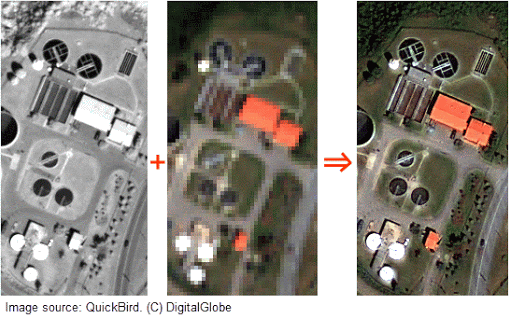
\includegraphics[scale=.7]{pansharpeningexample.png}
		\caption{Pansharpening example}
		\label{fig:pansh}
\end{figure}

Based on a convolutional neural network, a new pansharpening method has been proposed recently \cite{pnn}.
Using a degraded version of the PAN and MS images, the network's weights were trained to fuse the images, optimizing a reference index with the gradient descendent algorithm: the mean squared error. After the training, the same weights were applied to fuse the original PAN and MS images.
The purpose of this work is to improve the current methodology using the original PAN and MS images for a training with a no-reference index like QNR or HQNR indexes. Furthermore, the intention is to remove the error added using the degraded images that do not reflect the models were the pansharpening algorithm should be utilised.
In \cite{pnn} the code was written in python 2.7 using the Theano library. The Theano project has been not updated since 2018 \cite{theanorip}. For this reason, the project is incompatible with new Cuda libraries and NVIDIA drivers and many issues to run the training process on the GPU have been founded. To solve that, a new software has been created using TensorFlow. Tensorflow is a more modern and popular DeepLearning library maintained by Google that allow more compatibility with the newest libraries and a larger community helping the development in case of uncommon errors. As Theano does, Automatic Differentiation has been implemented by the new library \cite{tensorflowautoderiv}. Indeed, Automatic Differentiation can be defined as critical feature that allows writing differentiable functions and subsequently using them for the core algorithm of the neural network's backpropagation training: the gradient descendent algorithm. 


\chapter{Pansharpening state of the art}


According to the current methodology, the pansharpening techniques are divided into two main areas: component substitution (CS) and the multiresolution analysis (MRA). The techniques belonging to the first class consist in representing the MS and PAN in a different domain that can entirely split the spatial information from the spectral information. In this domain, the spatial information part of the MS image can be replaced with the PAN image. After this substitution, the MS image can be back-transformed in the original domain. Clearly, the less the PAN is correlated with the replaced component, the more distortion is introduced. The most famous techniques of this class are intensity-hue-saturation (IHS) \cite{ihs1} \cite{ihs2}, in which the images are represented in the IHS domain, principal component analysis (PCA) \cite{scaleinvariance1} \cite{pca2} and Gram-Schmidt (GS) spectral sharpening \cite{gs}. On the one side, those techniques preserve the PAN spatial information. On the other side they can produce a high spectral distortion. This is because PAN and MS are obtained in spectral ranges that only partially overlap. 

The second class of techniques, MRA, are based on the introducing of spatial details extracted from the PAN image into the up-sampled version of the MS. This approach promises a better spectral fidelity but often present spatial distortions.

The lack of the reference image is the principal issue in the evaluation of the pansharpening methods.
When a couple of images are fused, the result cannot be compared with anything else. The sensors used for the acquisition cannot reach alone both spatial and spectral resolution of the result. As the two models are different, the result cannot be compared with another image acquired with a different sensor.
For this reason, there is no universal measure of quality for the pansharpening. The scientific community common practice is to use the verification criteria that were proposed in the most credited work \cite{towaldetal}. This study defines two properties to use for the evaluation of the fused product: consistency and synthesis. The first means that the original MS image should be obtained with a degradation of the fused result.
The second property describe that the fused image should preserve both the features of each band and the mutual relations among them. The definition of an algorithm that accomplishes these properties and of an index that can guarantee the correct evaluation are an open problem. But, no matter what index is decided to use, the unavailability of a reference image is a huge problem and a visual inspection is always mandatory. There are two techniques that can be used as a workaround. The first is to reduce both the images given in input to the pansharpening algorithm and use the original MS image as a reference for the result evaluation. The downside of this method is the assumption of invariance between scales, which justifies that the same algorithm operates similarly at reduced scale. The cited hypothesis  is not always verified as documented here \cite{scaleinvariance1} \cite{towaldetal}. A second technique is the use of an index that does not require a reference image.


\section{CS}

The CS family is based on converting the MS image into a domain in which the spatial and spectral pieces of information can be better separated. In this domain, the component containing the spatial information can be replaced by the PAN image. The greater the correlation between the PAN image and the replaced component, the lower the distortion introduced by the fusion. For this reason, the histogram matching of the PAN with the component that contains the spatial part of the MS information is preliminarily performed.
After the substitution, the data can be represented in the original space with an inverse transformation. This approach is applied to the whole image in the same way. Techniques of this category have high fidelity regarding the fusion of spatial details and are fast and easy to implement. But as the acquisition spectrum of the sensors used to produce the PAN and MS image differ each other, the process may produce significant spectral distortions \cite{cs1} \cite{cs2}. 
In the studies \cite{cs3} \cite{cs4} \cite{cs5} \cite{cs6} \cite{cs7}, it was shown that, when a linear transformation is used, the substitution and fusion can be obtained without the explicit forward and backward transformation of the images but with a precise injection scheme. This scheme can be formalized according to the following equation:
 %
\begin{equation}
    \widehat{MS_k} = \widetilde{MS_k} + g_k(P - I_L), \qquad k = 1,\dots,N
    \label{cs}
\end{equation}
%
in which $k$ indexes the spectral bands, $g_k$ are the injection gains, $\widehat{MS_k}$ is the $k$-th band of the pansharpened image, $\widetilde{MS}_k$ is the $k$-th band of the MS image interpolated to the PAN scale and $I_L$ is the intensity component derived from the MS image according to the relation:
% 
\begin{equation}
    I_L = \sum_{i=1}^{N} w_i\widetilde{MS_i}
    \label{ilcs}
\end{equation}
%
The weight vector $w= [w_1,w_2, \ldots,w_k] $ is the first row of the forward transformation matrix and depends on the spectral overlap among MS channels and PAN.
 

\begin{figure}[t!]
\centering
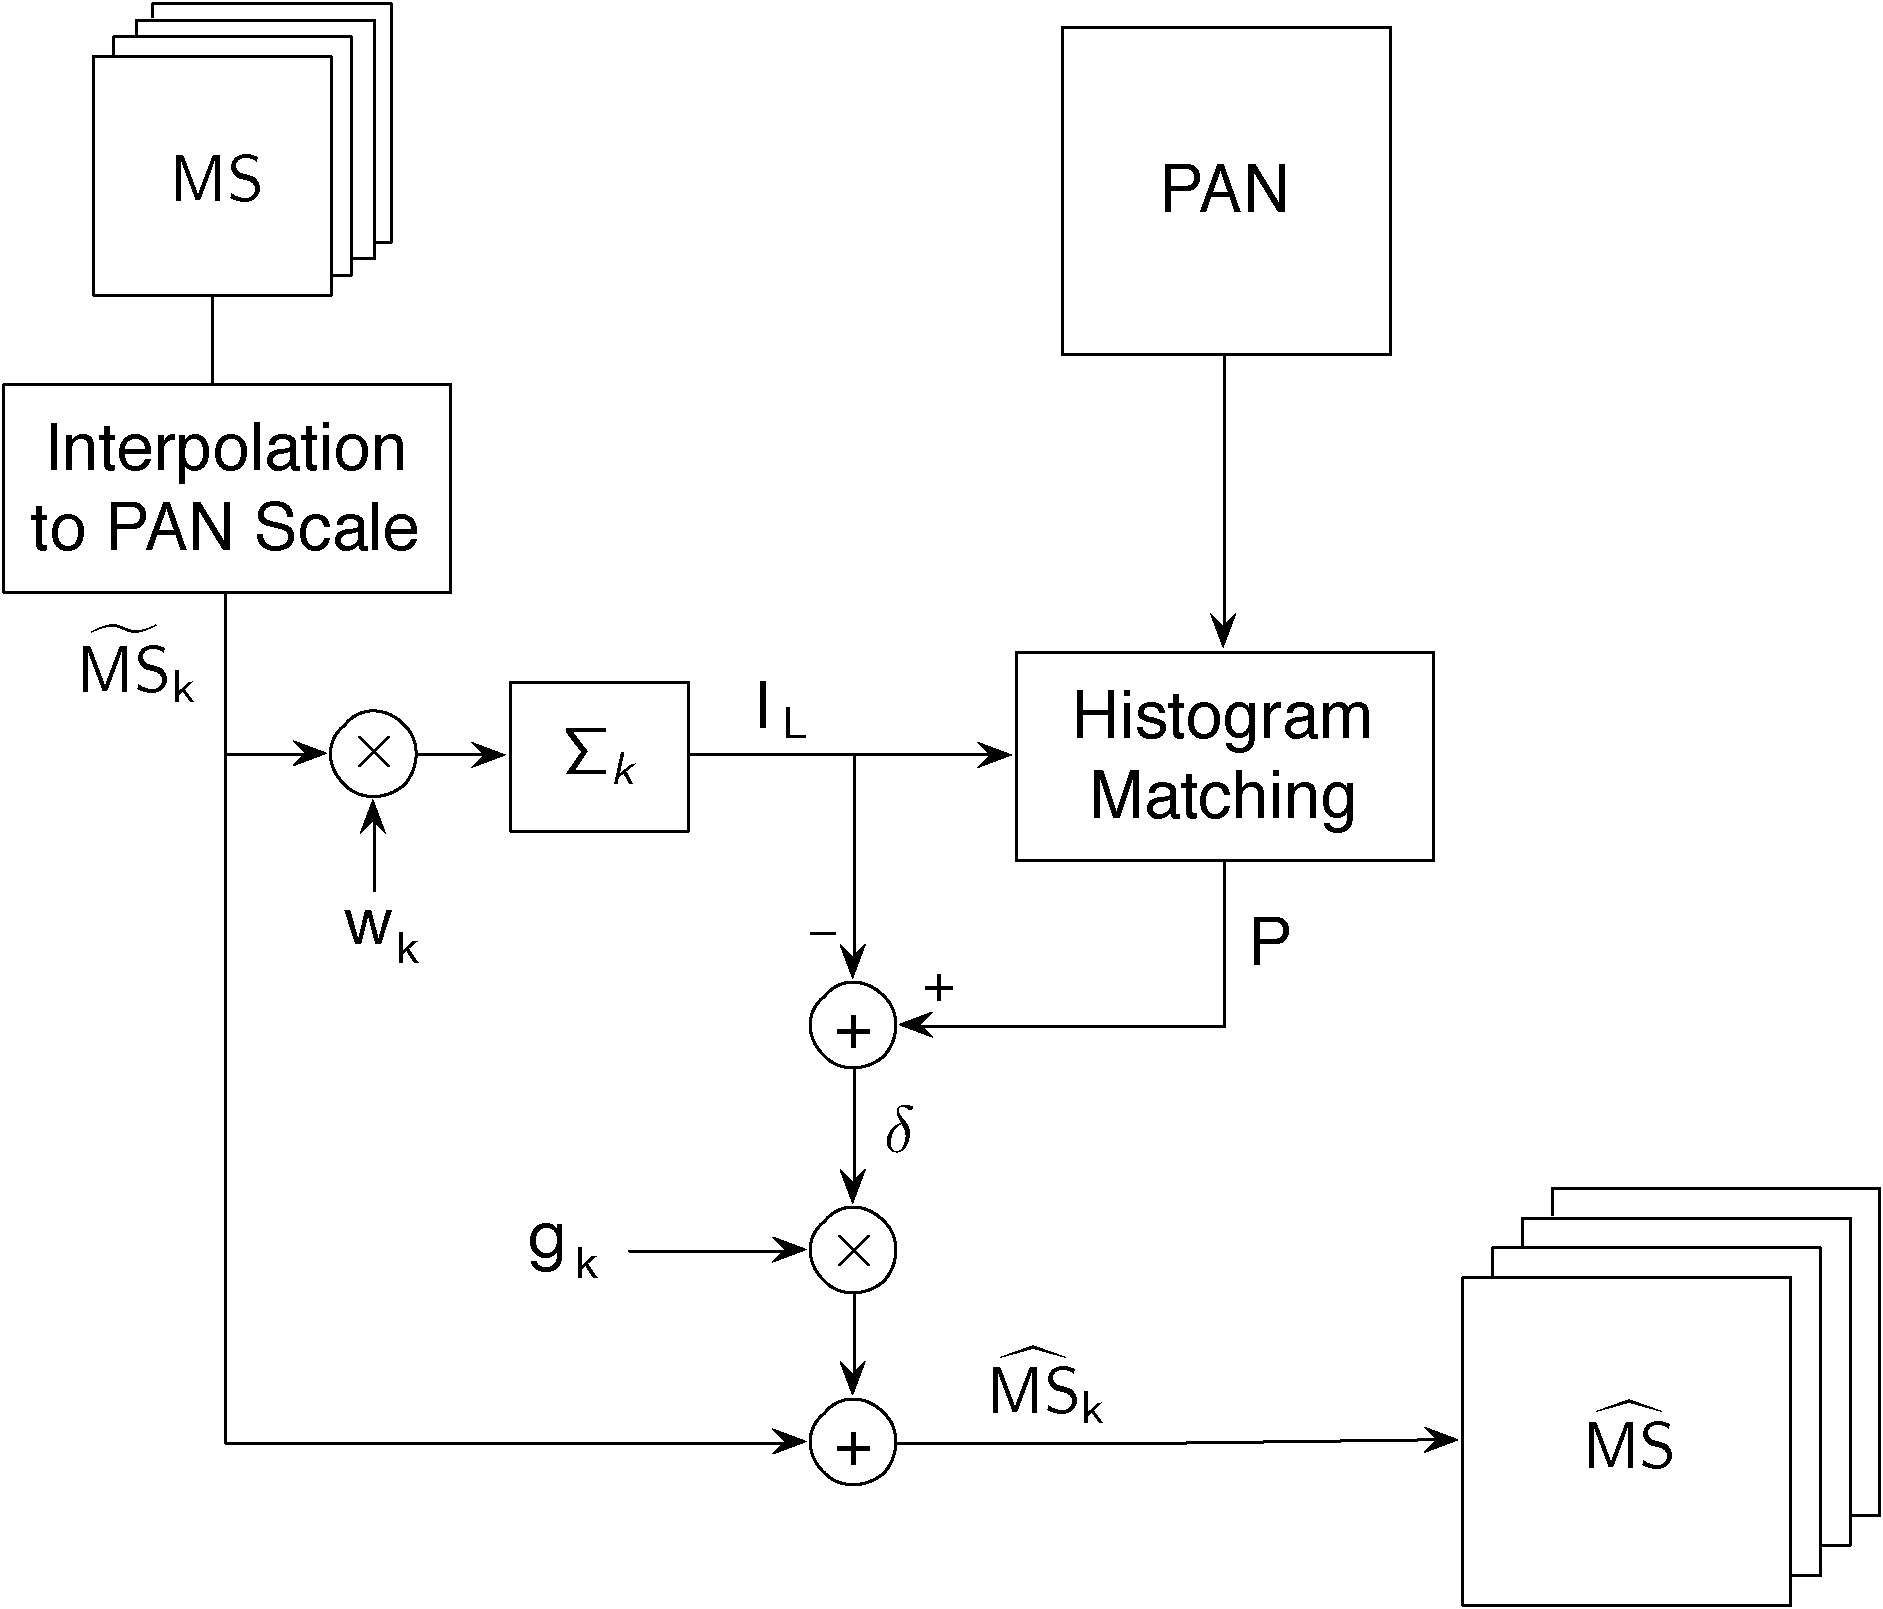
\includegraphics[width=\textwidth]{cs.png}
\caption{Flowchart of CS approach \cite{criticalComparison}}
\label{fig:csapproach}
\end{figure}


The CS approach procedure is illustrated in  Fig.~\ref{fig:csapproach}. Four important steps can be noticed: 
1) interpolation of MS image for matching the PAN scale; 2) calculation of $I_L$ using Eq.~(\ref{ilcs}); 3) histogram matching between PAN and intensity component; 4) details injection according to Eq.~(1).

The various CS techniques such as IHS \cite{ihs1,ihs2}, PCA \cite{pca2,changedetection} and GS \cite{gs,cs3} define different $w_{k,i}$ and $g_k$.

In the IHS pansharpening method is used the IHS transformation. This is the major limitation of this technique because it can transform only images in RGB and often the MS image has 4 or also 8 and more bands. As a workaround, the authors of paper \cite{cs6} has proved that GIHS, a generalization of the IHS transformation for more bands, can be formulated for any arbitrary set of nonnegative spectral weights as described in the following equation: 
%
\begin{equation}
    \widehat{MS_k} = \widetilde{MS_k} + \left(\sum_{i=1}^{N}w_i\right)^{-1}(P - I_L), \qquad 
    k = 1,\dots,N
    \label{cs2}
\end{equation}
%
in which $w_i$ are all equal to $1/N$ \cite{ihs1}.
With the injection gains defined such that:
\begin{equation}
    g_k = \frac{\widetilde{MS_k}}{I_L}, \qquad k = 1,\dots,N
    \label{csgk}
\end{equation}
%
$\widehat{MS_k}$ can be calculated as 
\begin{equation}
    \widehat{MS_k} = \widetilde{MS_k} \cdot \frac{P}{I_L}
    \label{csfinal}
\end{equation}
%
which is the known Brovey Transform. 

In the PCA pansharpening method, it is used the PCA transformation, also called Karhunen-Loeve transform. It is a linear transformation that can be implemented for a multidimensional image, so it is not limited as the IHS method, and consists into the projection of all the components along the eigenvectors of the covariance matrix. This means that each component is orthogonal and statistically uncorrelated from the others. The hypothesis introduced in this step is that the spatial information is concentrated in the first component, the component with the higher eigenvalue. The PCA can be implemented by using Eq.~\ref{cs}, in which $w$ is the first row of the forward transformation matrix; $g$ is the first column of the backward transformation matrix.

The GS transformation is a common technique used to orthogonalize a set of vectors in linear algebra.
First of all, the $\widetilde{MS}$ bands are organized in vectors to obtain a two dimensional matrix in which the columns are constituted by the bands organized as vectors. The mean of each band is subtracted from all the columns. The orthogonalization procedure is used to create a low-resolution version of the PAN image, i.e. $I_L$.  The last step is the replacement of $I_L$ with the histogram matched PAN before the inverse transformation. GS is a generalization of PCA in which PC1 may be any component and the remaining ones are calculated to be orthogonal with PC1. Also the GS procedure can be described by Eq.~\ref{cs} if $g_k$ is defined as:
%
\begin{equation}
    g_k = \frac{\operatorname{cov}(\widetilde{MS_k}, I_L)}{\operatorname{var}(I_L)} , \qquad k = 1,\dots,N
    \label{gsgk}
\end{equation}
%
in which $\operatorname{cov}(\cdot,\cdot)$ is the covariance between two images and $\operatorname{var}(\cdot)$ is the variance.
There are several version of this technique that differ on how the $I_L$ is
created. The simplest way is to set $w_i = 1/N$. This version is called 
GS mode 1~\cite{gs}. It was proposed also an $adaptive$ version of this mode 
called GSA in~\cite{cs3} in which $I_L$ is generated by a weighted average of 
the MS bands. Another technique defined in \cite{gs} and called GS mode 2 
suggests to generate the $I_L$ by applying a low pass filter to the PAN image. 
This last step leads the GS mode 2 that belongs to the MRA class of techniques.

Another noteworthy technique is described in \cite{cs7} that introduces the concept of 
\textit{partial replacement } of the intensity component. An intensity
image is created  for every band of the MS from the PAN image; it is calculated with the following equation:
%
\begin{equation}
    P^{(k)} = CC(I_L, \widetilde{MS_k}) \cdot P + (1 - CC(I_L, \widetilde{MS_k})) \cdot 
    \widetilde{MS_k^{'}}
    \label{pk}
\end{equation}
%
in which $\widetilde{MS_k^{'}}$ is the $k$-th MS band histogram-matched to PAN and CC is the
correlation coefficient.
$I_L$ is defined using in Eq.~\ref{ilcs} a vector $w$  obtained with a linear regression of $\widetilde{MS_k^{'}}$
on $P_L$, the degraded version of the PAN.
The injection gains are the result of:
%
\begin{equation}
    g_k = \beta \cdot CC(P_L^{(k)}, \widetilde{MS_k}) \cdot 
    \frac{std(\widetilde{MS_k})}{\frac{1}{N}\sum_{i=1}^N std(\widetilde{MS_i}))} L_k
    \label{gkpk}
\end{equation}
%
$\beta$ is empirically tuned and is a factor that normalizes the high frequencies.
$P_L^{(k)}$ is a low-pass-filtered version of  $P^{(k)}$,  and $L_k$ is an adaptive factor 
that removes the local spectral instability error between the synthetic component image 
and the MS band defined as:
%
\begin{equation}
    L_k = 1 - |1 - CC(I_L, \widetilde{MS_k})\frac{\widetilde{MS_k}}{P_L^{(k)}}|.
    \label{lk}
\end{equation}
%

\section{MRA}

In the MRA class of techniques, the pansharpened image is defined as:
%
\begin{equation}
    \widehat{MS_k} = \widetilde{MS_k} + g_k(P - P_L), \qquad k = 1,\dots,N. 
    \label{mra}
\end{equation}
%
$P - P_L$  is the operation performed to obtain the high-frequency details of the PAN image. 
The algorithm to create the $P_L$ and the chosen $g_k$ weights differentiate the MRA 
pansharpening techniques of this class.

\begin{figure}[t!]
\centering
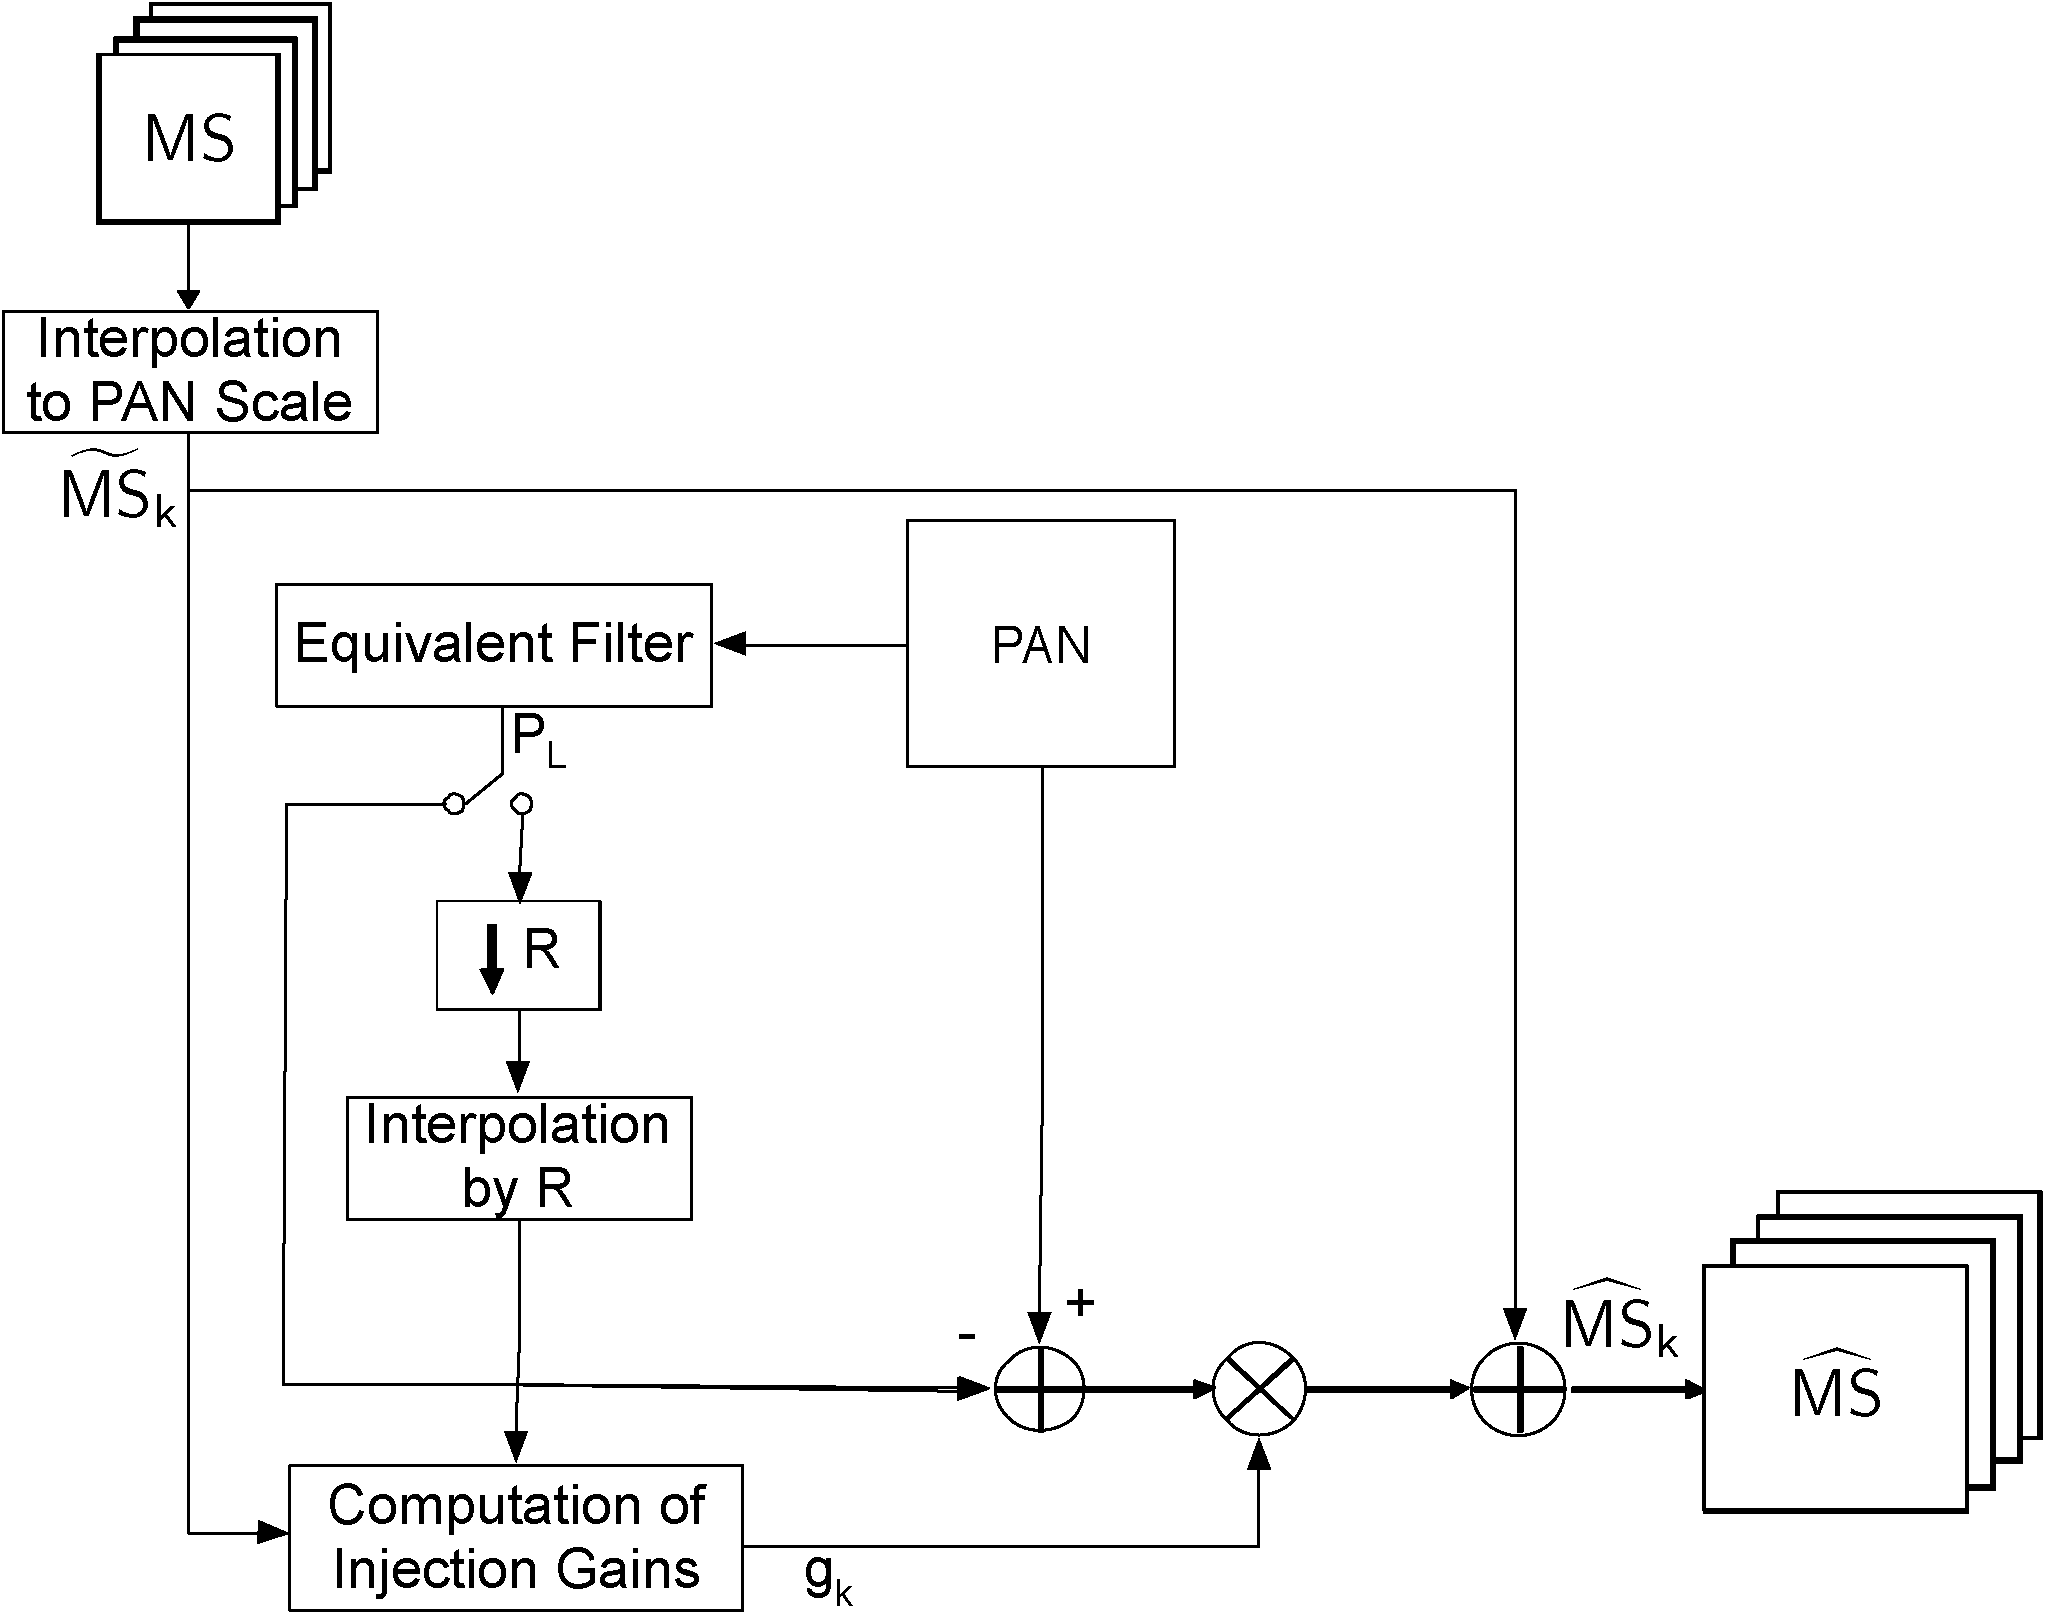
\includegraphics[width=\textwidth]{mra.png}
\caption{Flowchart of MRA approach \cite{criticalComparison}}
\label{fig:mraapproach}
\end{figure}

However, in general, all the techniques follow the algorithm described in Fig.~\ref{fig:mraapproach}. 
First of all, the MS image is interpolated to the PAN scale.
The second step is to calculate $P_L$, the low pass version of PAN obtained by means of an equivalent filter.
The vector of injection weights $g_k$ can be computed using the $\widetilde{MS_k}$ in combination with $P_L$.
Interpolation is less crucial in MRA respect to CS methods.
A method to produce the $P_L$ image consists in applying a low pass filter $h_{LP}$ to the PAN image $P$.
So Eq.~(\ref{fig:mraapproach}) can be rewritten as:
%
\begin{equation}
    \widehat{MS_k} = \widetilde{MS_k} + g_k(P-P*h_{LP}), \qquad k=1,\dots,N
    \label{mra1}
\end{equation}
%
where $*$ is the convolution operation.
A more general method to obtain the $P_L$ is called \textit{Pyramidal Decompositions} and the number of 
filterings can be one or more. A filter type that proves to be a good choice is a Gaussian filter that closely 
matches the sensor MTF. A noteworthy option is the MTF-GLP with a context-based decision (MTF-GLP-CBD) \cite{mtfglp}
where the injection gains are defined as follows: 
%
\begin{equation}
    g_k = \frac{cov(\widetilde{MS_k}, P_L^{(k)})}{var(P_L^{(k)})}
    \label{mragk}
\end{equation}
 It is context-based because it can be applied on nonoverlapping image patches to improve the quality of the final product.

\section{Quality Assessment}
As explained above, the lack of a reference image is the main limitation. The community has proposed two assessment
procedures as a workaround. The first procedure consists in using the images at a lower spatial 
resolution and use the original MS image as a reference. However, the output of an algorithm can have 
different performance at different scales, as it is showed in~\cite{perfdiffscale}.
This because the performance assessment depends intrinsically to the image scale, 
mostly in case of pansharpening methods that apply spatial filters.
The second procedure consists in using non-reference quality indexes. 
Both types of procedures require also a visual inspection for spectral distortions and spatial details.

The Wald's protocol is composed by three requirements:
\begin{enumerate}
	\item $\widehat{MS_k}$ degraded to the original MS scale should be as identical as possible to the $MS_k$.
    \item The fused image $\widehat{MS_k}$ should be as identical as possible to the $MS_k$ that the sensor would acquire at the highest resolution
    \item The MS set of synthetic images $\widehat{MS} = {\{\widehat{MS}\}_{k=1,\dots,N}}$ should be as identical as possible
    to the MS set of images $HRMS = \{HRMS\}_{k=1,\dots,N}$ that the corresponding sensor would observe at the highest resolution.
\end{enumerate}

In the previous definitions HRMS is the reference image.
For a reduced-resolution assessment, the filter choice for the downsampling is crucial in the validation. 
A bad filter choice results in an image degradation that does not reflect the 
sensor characteristics at a lower scale. So the algorithm, after the degradation, is applied to
images that reflect the wrong sensor model. This means that the same algorithm can have a more different result at the original and lower scales. On the contrary, with a good filter that preserves the sensor characteristics at the lower resolution, the algorithm has much more possibility to reflect the quality of the original resolution.
Indeed, the filter used for the MS degradation should simulating the transfer function of the remote sensor and so, it should match the sensor's MTF~\cite{mtfsensor}. 
Similarly, the PAN image has to be degraded in order to contain the details that would have been seen if the image were acquired at the reduced resolution.
The fused image obtained from the degraded PAN and MS, can be evaluated different indexes using the MS as a reference image.

The Spectral Angle Mapper (SAM) is a vector measure that is useful to evaluate the spectral distortion.
In simple terms, denoting by $I_{(n)} = [I_{1,{n}}, \dots , I_{N,{n}}]$ a pixel vector of the MS image, with $N$ bands,
the SAM between the corresponding pixel vectors of two images is defined as:
%
\begin{equation}
    SAM(I_i, J_i) = arcos(\frac{<I_i, J_i>}{||I_i|| || J_i||})
    \label{sam}
\end{equation}
%
$<I_i, J_i>$ is the scalar product and $||I_i||$ is the vector $l_2$-norm. 
Applying this equation to every pixel results in a so-called SAM map.
Averaging all the pixel of the SAM map returns the SAM index for the whole image.
The optimal value of the SAM index is 0.

RMSE is used to calculate the spatial/radiometric distortions.
It is defined as:
%
\begin{equation}
    RMSE(I,J) = \sqrt{E[(I-J)^2]}
    \label{rmse}
\end{equation}
%
The ideal value of RMSE is zero and is achieved if and only if $I = J$.
But it is not an efficient index because it is not considered the error for each band, but is global.
So, to better measure the error for each band, the ERGAS index is used. 
The ERGAS index evaluates the RMSE error with a different weight for each band.
%
\begin{equation}
    ERGAS = \frac{100}{R} \sqrt{\frac{1}{N} \sum_{k=1}^N\left(\frac{RMSE(I_k, J_k)}{\mu(I_k)}\right)^2}
    \label{ergas}
\end{equation}
%
Obviously, the ERGAS is composed of a sum of RMSE, so the optimal value is also 0.
Another important index is the Universal Image Quality Index (UIQI) or also called Q-index, proposed in \cite{uiqi}.
Its expression is:
%
\begin{equation}
    Q(I,J) = \frac{\sigma_IJ}{\sigma_I \sigma_J} \frac{2 \bar{I}\bar{J}}{\bar{I}^2 + \bar{J}^2} 
    \frac{2 \sigma_I \sigma_J}{(\sigma_I^2 + \sigma_J^2)}
    \label{q}
\end{equation}
%
where $\sigma_{IJ}$ is the covariance of $I$ and $J$, and $\bar{I}$ is the mean of $I$.
The first fraction represents an estimation of the covariance, the second is a difference in the mean luminance
and the third is the difference in the mean contrast.
The Q-index varies in the range $[-1, 1]$ with 1 as the optimal value.


Q4 is an extension of the UIQI for images with 4 bands \cite{q4}. 
Let $a$, $b$, $c$ and $d$ denote the radiance values of the given image pixel in four bands, and let the quaternions:
%
\begin{equation}
    z_A = a_A + ib_A + jc_A + kd_A
    \label{za}
\end{equation}
%
\begin{equation}
    z_B = a_B + ib_B + jc_B + kd_B
    \label{zb}
\end{equation}
%
The Q4 is defined as :
%
\begin{equation}
    Q4 = \frac{4 | \sigma_{z_A z_B}| \dot |z_A| \dot |z_B|}{(\sigma_{z_A}^2 + \sigma_{z_B}^2 (|z_A|^2 + |z_B|^2))}
    \label{q4}
\end{equation}
%
If eventually, the bands are more than 4, the Q4 can be replaced with Q average.

An index used for the validation at full-resolution is the Quality with no reference (QNR) index \cite{qnr}.
It is defined by the following equation:
%
\begin{equation}
    QNR = (1-D_{\lambda})^\alpha (1 - D_S)^\beta
    \label{qnr}
\end{equation}
%
$\alpha$ and $\beta$ are two coefficients which can be tuned to weight more
the spectral or the spatial distortion, respectively.

The maximum theoretical value of the index is 1 and is reached when $D_\lambda$ and $D_S$ are 0.
The spectral distortion is calculated with $D_\lambda$ using this equation:
%
\begin{equation}
    D_\lambda = \sqrt[P]{\frac{1}{N(N-1)} \sum_{i=1}^N \sum_{j=1, j \neq i}^N |d_{i,j}(MS, \widehat{MS}|^P)}
    \label{dl}
\end{equation}
%
where $d_{i,j}(MS, \widehat{MS}) = Q(MS_i, MS_j) - Q(\widehat{MS_i}, \widehat{MS_j})$, $\widehat{MS}$ is
the fused image and $p$ is a parameter typically set to one \cite{qnr}.
The objective is to create an image with the same spectral features of the original MS image.

The spatial distortion is calculated by:
%
\begin{equation}
    D_S = \sqrt[q]{\frac{1}{N} \sum_{i=1}^N |Q(\widehat{MS_i}, P) - Q(MS_i, P_{LP})|^q}
    \label{ds}
\end{equation}
%
where $P_{LP}$ is the low-resolution PAN image at the same scale of the MS image and $q$ is usually set to one \cite{qnr}.

Khan protocol \cite{khan} extends the consistency property of Wald's protocol.
The pansharpened image is considered as a sum of a lowpass term plus a high pass term.
The lowpass term is the original interpolated low resolution MS image and
the highpass term corresponds to the spatial details extracted to the PAN and injected into the MS image.
A Gaussian model of the sensor's MTF is used to build the filters. The similarity between the lowpass component and
the original MS image can be calculated using the Q4 index or any other similarity measure for images with more bands.
The similarity between PAN and the spatial component is measured as the average of UIQI calculated using the PAN and each band of MS.
The same similarity is calculated also between the original MS and the degraded version of the PAN.

The QNR and the spectral distortion of Khan's protocol can be combined to yield another quality index, the HQNR \cite{hqnr}:
%
\begin{equation}
    HQNR = (1 - D_\lambda^{(K)}) (1 - D_s) 
    \label{hqnr}
\end{equation}
%
in which $D_\lambda^{(K)}$ is :
%
\begin{equation}
    D_\lambda^{(K)} = 1 - Q4(\widehat{M_L}, M)
    \label{dlhqnr}
\end{equation}
%
The $ \widehat{M_L} $ is the fused image degraded to the resolution of the original MS image. 

\newpage

\chapter{Pansharpening applications of Deep Learning}

\section{Introduction}

Early works in the field of Deep Learning have been made in the 1940s with the Perceptron \cite{perceptron} and in the 60s with the invention
of backpropagation that is the most commonly used algorithm in the present day to train a Neural Network.
The Neural Network is a model constituted by several Perceptron or also called neurons divided into different layers that give the 
ability to learn, extract and distinguish different features from the data given in input.
To learn these capabilities, the network should be subject to a training phase that requires an incredible amount of
computational power.
Indeed, in the beginning, this type of algorithm was discarded because the computes in the 60s was
not powerful enough and there wasn't a great data availability. 

LeCun in 1989 for the first time used a backpropagation algorithm to train a convolutional neural network, a particular
type of networks constituted from different convolutional layers to classify handwritten digits.

These days, the data collected with the internet, the incredible amount of computational power exhibited
by data centers and GPUs, the performance of this type of algorithm and a large number of applicative fields,
has encouraged the growth of Machine Learning and in particular, Deep Learning. 

The training is a phase in which the model learns from new data and can differ for the type of issues that the model should solve.
Most of the cases, the model gives a prediction and the result is compared with a reference. It is calculated the error between the
output of the prediction and the reference and this error is propagated in all the neurons of the model. 
This error modify the weights of all the neurons so that the next prediction for the same input it will much similar to the
reference output. 
How this error is calculated and what means "similar" is established by the loss function that calculates the error.
The backpropagation uses the Gradient Descendent algorithm, that it allows the network 
to understand how to change the weights to minimize the loss.
To use the Gradient Descendent, the loss function must be differentiable so that,
the gradient operator can be applied more times.
Many layers the net have, many times the algorithm apply the gradient to the function.

\section{Neural Networks}

\subsection{Perceptron}

Essentially a perceptron is an element in which, the output is a result of a weighted sum
of the inputs. There is only one output but can be more inputs as described in the Fig.~\ref{fig:perceptron}. 
A perceptron uses only one linear or non-linear activation function. In the following paragraph it will discuss what is an activation function.
With a non-linear transfer function, perceptron can build a nonlinear plane separating data points of different classes.
In 1969, it was proved that the perceptron itself may fail in certain simple tasks for example
the separation of a plane described by the XOR function. 
But 3 perceptron organized in 2 layers can separate an XOR plane.
This opened up the development of multi-layer models and subsequently, for training optimization for specific
applications, the creation of the different type of layers.

\begin{figure}[t]
    \centering
    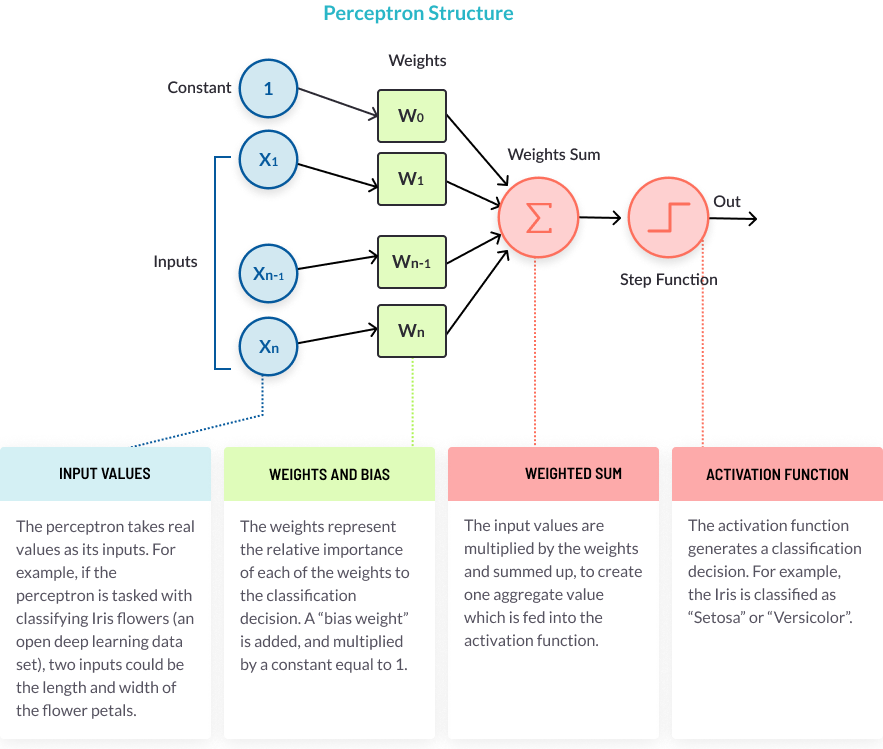
\includegraphics[width=\textwidth]{perceptron-structure.png}
    \caption{Perceptron in detail \cite{percepimage}}
    \label{fig:perceptron}
\end{figure}

\subsection{Activation Function}

An activation function is used to transform the weighted data (input multiplied weights) 
in outputs, in deep learning often a non-linear transformation.
Indeed, using a non-linear transformation, we create new relationships between the points
and this consent to the machine learning model to create increasingly complex features with every layer.
Features of many layers that uses pure linear transformations can be reproduced by a single 
layer that use a non-linear function. 
Most common activation functions is the rectified linear function or also colled ReLu that
can be described as $y = max(0, x)$. The gradient is always x when the value of x is positive, 
and 0 when negative. This means that during the training, negative gradients will not update the weights.
Gradient equal 1 means that the training will be much faster compared with other activation functions
like logistic sigmoid.

\subsection{Layers}

\begin{figure}[t]
    \centering
    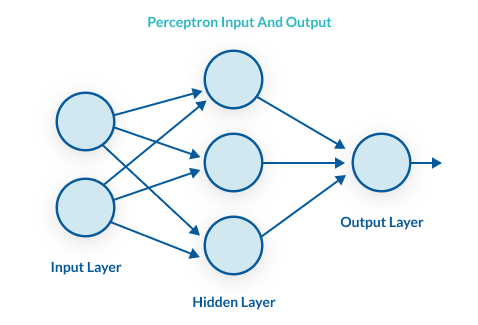
\includegraphics[scale=.5]{multilayer-perceptron.png}
    \caption{Multilayer architecture example \cite{percepimage}}
    \label{fig:multilayer}
\end{figure}

The DL network can have different layers type that differ in how the perceptrons inside them are organized and 
how they modify their weights during the training. 
A layer of neurons can be expressed as a function, mostly non-linear, that apply a transformation of the input into the output as described in Fig.~\ref{fig:multilayer}.
The first created layer was the dense layer in which all the neurons of a dense level are connected
with all the neurons of the next layer. Every neuron has his weights that are tuned during the training phase
and this generates very fast a large number of weights to train, so the necessity of a larger
dataset and a longer time for the training. 
The DL model is capable to extract and recognize features in the data as complex as the complexity of the model growth.
A layer that gave an important improvement in computer vision applications is the
convolutional layer, a layer that can apply different filters to the data at the same time.
Commonly, several convolutional layers at the start of a neural network are used to extract features from an image. Features that can be 
in a second phase, analyzed by a different type of layer, for example, a dense layer that has the characteristic to have a lot of neurons with different weights
and so can learn different type of features (Fig.~\ref{fig:featuresextract}).
The filters weights are learned in the training and don't matter how big is the image given in input,
the same filters are applied for the entire input dimensions and the perceptions that constitute the layer,
share the same weights. So, respect to a dense layer, the convolutional layer has a lower weights count. 
This means that a convolutional layer is much faster to train and also allocate a minor amount of memory.
Different layers in sequence can extract features more and more complex. 
LSTM and GRU layer was created to give to the model the capability to predict using a sequence of data such as video or audio.
Other layers were created to optimize the training like the pooling layer, max-pooling layer and dropout.


\begin{figure}[t]
    \centering
    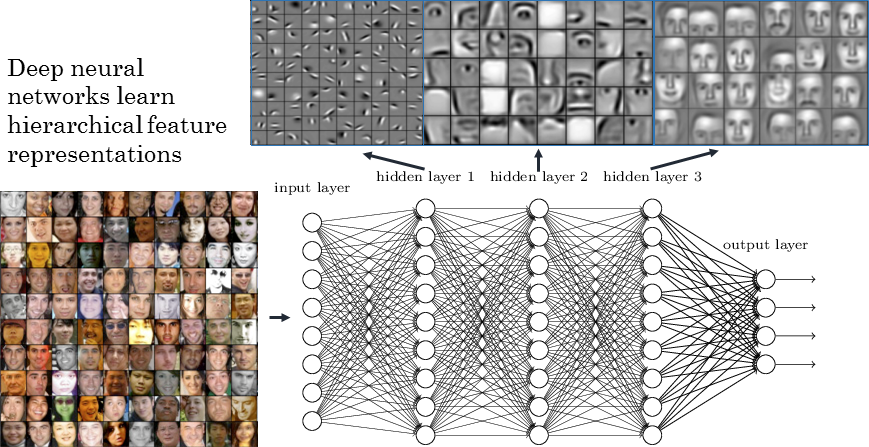
\includegraphics[scale=.5]{layers-features.png}
    \caption{Feature extraction of a deep model \cite{featuresextract}}
    \label{fig:featuresextract}
\end{figure}


\section{The Deep Learning Paradigm}

Deep Learning is a subfield of Machine Learning focalized in the study of deep neural networks.
The model architecture is made in such a way to extract features from the data and after lean from them.
In this, the Deep Learning field differs from the other Machine Learning techniques in which they were focused, before, only on
learning from handcrafter features. These are much more complicated to tune because require a high knowledge
of the data structure used in the particular context. In the DL, the net is trained also for this task, but the net architecture
is more complex.
Deep Learning gave a strong impulse to the development of very efficient algorithms in the computer vision field. 
Indeed, these days there are a lot of tools on the internet that simplifies the use of complex models trained to 
recognize hundreds of objects in an image. Also, there is the possibility to tune the net to recognize a custom object.
This can be done with a technique called fine-tuning. 
The fine-tuning is based on the concept (described also in Fig.~\ref{fig:dl-architecture}) that the initial layers of a model, 
in computer vision always convolutional layers, are trained to extract features from the input. 
This features will be used by the final layers of the model for the classification for example or for the target task of the model. The idea of fine-tuning is to reset the weights of the final layers so that the model, from the same features extracted, can classify different objects. With this technique is not necessary to train the model for days using very large datasets. 
\begin{figure}[t]
    \centering
    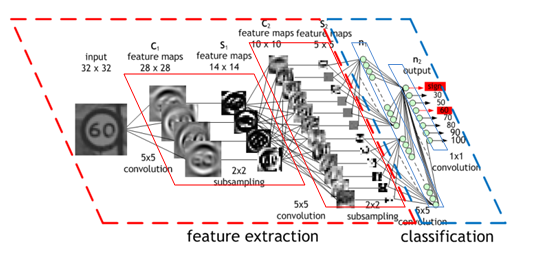
\includegraphics[scale=1.2]{dlarchitecture.png}
    \caption{Image by Maurice Peemen}
    \label{fig:dl-architecture}
\end{figure}


\newpage

\section{Pansharpening Applications}

Recently it was proposed in \cite{pnn} a new pansharpening method based on a convolutional neural network.
It was specialized a network built for super-resolution \cite{superesolution} to accomplishes the 
pansharpening task.
It was built three different models for GeoEye1, IKONOS and WorldView2 sensors. This because the net weights 
can be specialized to predict the sensor characteristics and give better performance. 
Not only the weights but also the layers are slightly different from each other because the authors run different 
test for each sensor to increase performance.
An important issue in this field is that it's difficult to found good images because of the high cost for a high-resolution images.
For this reason, it can't be built a deep network because became hard to train. The authors choice was to use three convolutional layers of architecture illustated in Fig.~\ref{fig:dl-pnn}. Using only convolutional layers have also the advantage that no matter the number of columns and rows
of the images, the model fits the images dimensions and it can execute the pansharpening on anyway. What matters is the number of MS channels.
The downside of convolutional layers is that reduce the image dimensions layer by layer because essentially, this type of layer
apply a conlution between the input and some filters of a pre-determined kernel size without adding padding.

\begin{figure}[t]
    \centering
    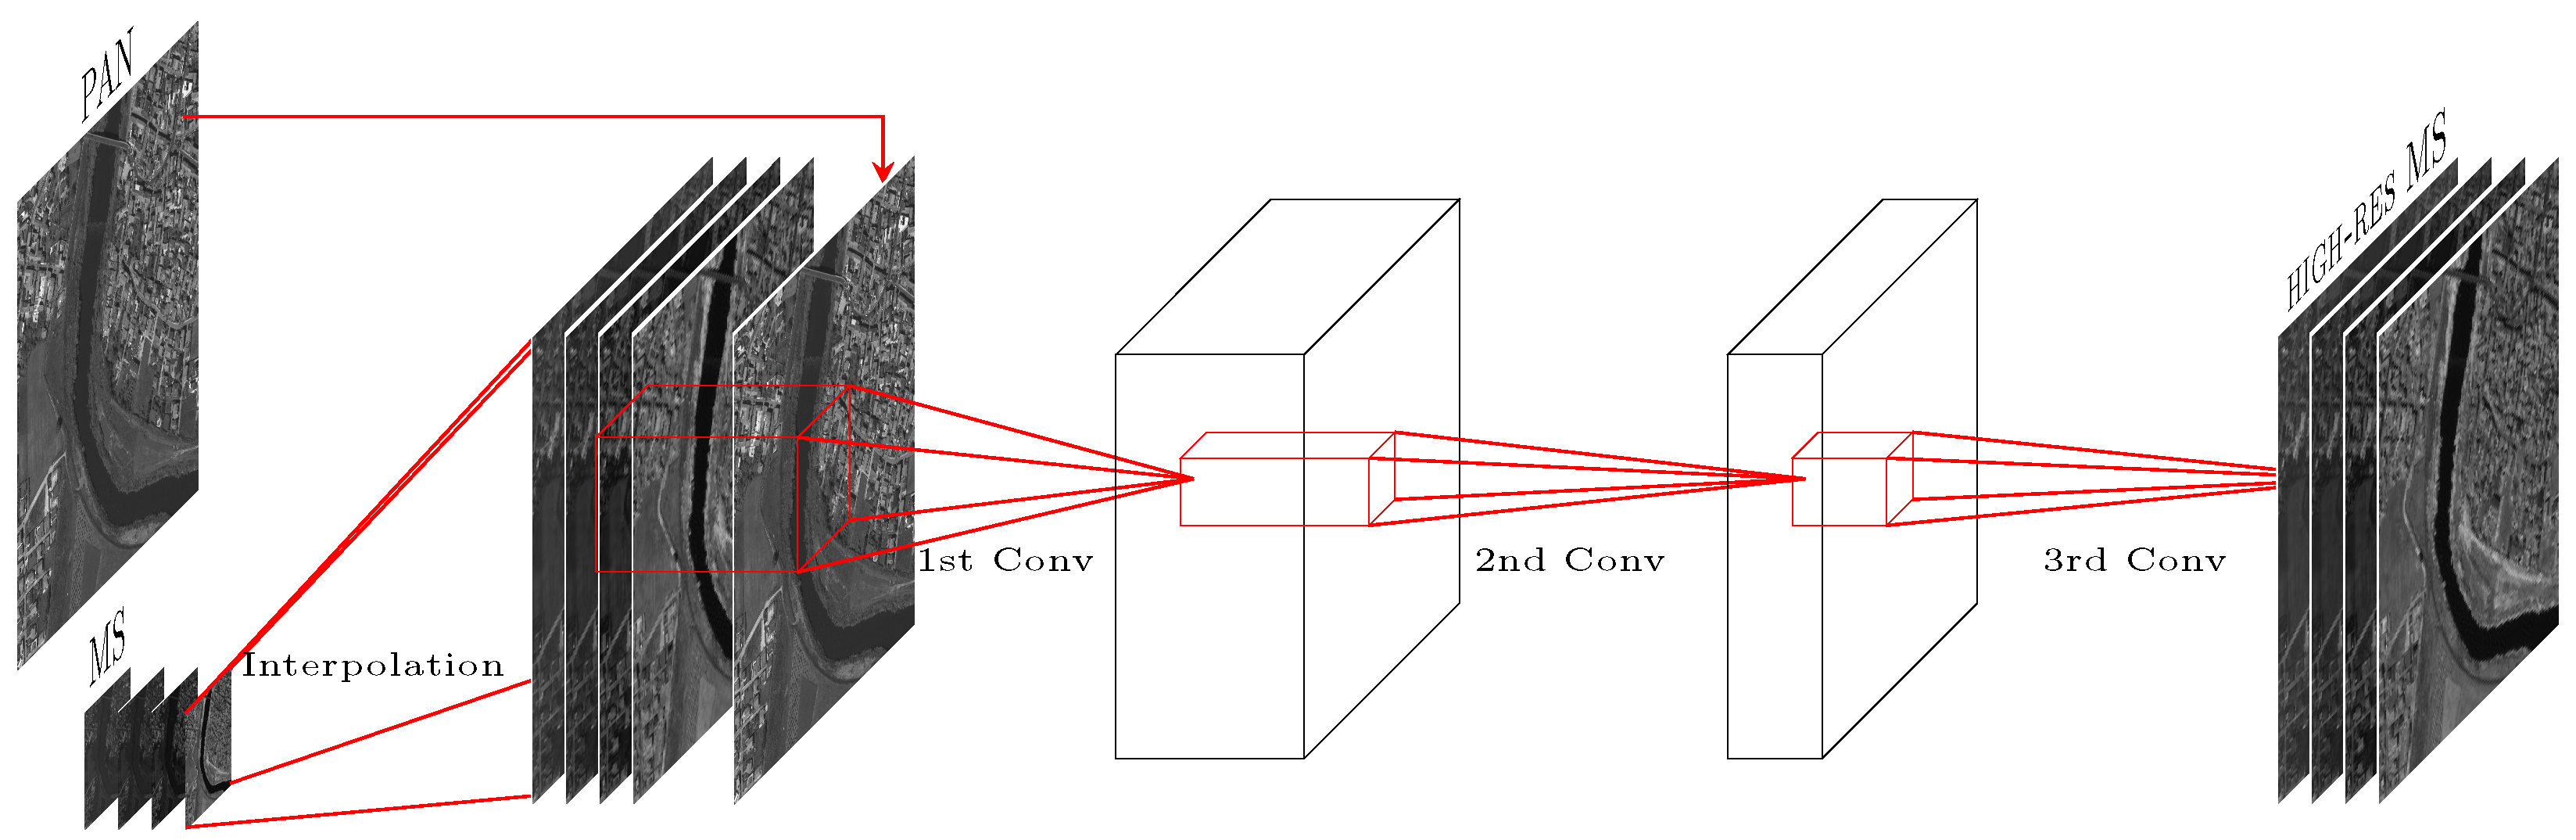
\includegraphics[scale=.8]{dl-pnn.png}
    \caption{CNN architecture for pansharpening\cite{pnn}}
    \label{fig:dl-pnn}
\end{figure}

\newpage

The training phase showed in Fig.~\ref{fig:pnn-training} uses a reference approach in which the images are downsampled and fused. 
After the downgrande, the $P_L$ image is appended to the MS downgraded and given in input to the model.
The MSE error between MS and the fused image is calculated and this error is used for the training of the weights.

\begin{figure}[t]
    \centering
    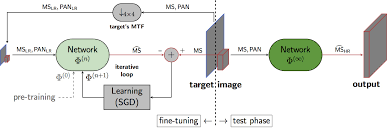
\includegraphics[scale=.9]{pnn-training.png}
    \caption{Training and Test\cite{pnn2}}
    \label{fig:pnn-training}
\end{figure}

An improvement illustrated into the paper was to append also some radiometric relevant indexes  for the applications
to adding information abound the image. It is showed that the network avoids learning this indexes that was already
provided and could focus to learn other information.
Another important step introduced in \cite{pnn2} is to run a fast session of fine-tuning before the 
application of the model to an image with the same procedure of the training.
With the fine-tuning, the net can learn to fuse the new image in a downgraded version.
This can train the network also for the new image and produce better performance.
But, as described in the conclusion of \cite{pnn2}, Full-resolution quality,
remains an open issue. Performance in downsampling domain is relatively relevance and
no-reference measures in training can have a major impact.
Another noteworthy downside of this method is that with misaligned images, the model is trained
with a fraction of the misalignment depends on the scale ratio between PAN and MS. 
This is an example that the degradation changes the sensor model in which we want to apply the pansharpening.

\newpage

\chapter{Proposed Solution}

\section{Introduction}

In this chapter will be described the concept of our solution and all the steps and issues encountered.
The main goal it was to select a correct loss function and implement it using modern tools.


\section{Loss Function Issue}
In general, deep learning models should not be specialized too much for the training set, 
because the model could have worse performance in real applications in which the net is not trained.
To avoid this situation, is necessary to create a validation set during the training. The validation set is a dataset
in which there are data that the net is not trained for. Performance on the validation set are more similar to real performance.
To generate a reference image, necessary for the quality assessment, it was downsampled an MS and PAN.
The original MS it was used as Ground Truth (GT) and the downgraded version will be called MS and PAN for simplicity.
To build the training set for the reduced resolution method, selected an image to performe the fine-tuning, it was used the downgraded version of PAN and MS with
the goal for the model to reproduce the MS. At every epoch, the PAN and MS were used 
to produce a fused image with the updated weights and compared with the GT and so, these images constitute a validation set. 
This procedure can give a real performance assessment of the whole model.
During the training, the training set have always better performance because the model is optimizing the 
error of these data. Only the performance of the validation set are really important. 

In the fine-tuning, it is noticed that some images have worse performance with the updated weights 
respect to the original ones without fine-tuning.
These because the model is fine-tuned with the downgrade version of the original image in which it should be performed the fusion.
The models in general are not scale invariance and downsampling the input does not guarantee similar performance like using the original images
as described also in the previous chapters.

The thesis' aim is to change the training process using the MS and PAN combined with a no-reference index 
and compare the results with the reduced resolution method. 
The degraded images were given in input to the two methods and the result was compared with the reference, the original image.
With the RR method ( reduced-resolution ), the inputs were downgraded another time for the fine-tuning, 
but with the NOREF method ( no reference ), the inputs were just used for the training with a no-reference loss function.
At every epoch, reference indexes like SAM, ERGAS and Q and also no reference index QNR and HQNR were calculated  between the images and the original image.
These indexes were calculated with the MatLab toolbox functions provided by \cite{criticalComparison} using the MatLab engine 
for python \cite{matlab}.


\section{Automatic Differentiation}
In mathematics, the automatic differentiation is a set of techniques to efficiently calculate, with a computer, the gradient of a function.
Every computer program executes a sequence of elementary operations. To calculate the gradient of a function,
most autodiff systems explicitly split the operations in a simplier ones and build a computation graph.
Each node of the graph have some attributes like value, primitive operation and parents.
For each primitive operation, it must be defined a Vector-Jacobian Product (VJP), a product based on the Jacobian
that is the matrix of partial derivatives. Combining all the VJP of all the nodes return the value of the gradient.

\section{Tensorflow and custom loss function implementation}
Tensorflow is the most famouse machine learning and deep learning tool that implement the automatic differentiation.
To define a custom loss function, Tensorflow provide an API. This API, define all the operations betweens Tensors that are the basic datatype of all operations in Tensorflow.
Tensors in this algorithm stage have no values, but only sizes and other attributes.
Only during the training, when the gradient is calculated layer by layer, the tensors acquire a value.
This allow to validate all operations before the actually computation and compile these safely.

After the definition of the custom loss function, at runtime Tensorflow translate the python code in C/C++ for efficience purpouse, compile it, and build the computation graphs.
Also, tensorflow from a couple of years integrate on it Keras, another framework that simplify the creation of the model with 
all common layers well-defined into Classes.
To create a model it is only necessary to create a $Model$ class.
And it's possible to add a layer using $model.add(Layer(args))$.
$Layer$ is the corresponding class of the layer and args are the arguments like the input shape, the number of filters that the layer should have and so on depends on the class. 
Use such a widespread framework has the advantage of having a large community that can help in difficult situations but 
also a much larger compatibility on Operating Systems, GPU and hardware in general.

\subsection{Loss Function}

To build the first loss function, it was used a QNR approximation. 

\begin{equation}
    f(x) = 1 - \widetilde{QNR}
    \label{loss}
\end{equation}
%
where $\widetilde{QNR}$ is the approximated QNR.

The $D_s$ and $D_\lambda$ were calculated using the Qavg that is the average of Q evaluation for each band. The Q was calculated considering the whole image and not
dividing it into small patches.
With this loss function, the result after the training presents a lot of negative values and also after a clip
by values of the image with 0 and 1 as minimum and maximum, the performance was unsatisfactory ( results illustated in the Chapter \ref{chap4}).
This because the model want to minimize the loss functions and so, maximize the QNR considering (25) no matter 
the sense of output values.
After some tests, it was considered to solve this problem using a different $D_s$, the $D_sreg$ \cite{dsreg} 
and migrate to an approximation of HQNR instead of the QNR.
It was discovered that it's really difficult to manipulate quaternions and hypercomplex numbers in TensorFlow in such
a way that the function remains differentiable so, the exactly HQNR it was impossible to implement.  
Also a different kind of $D_\lambda$ was implemented because the first one used by the original 
QNR did not reflect great performance according to the scientific community and the author itself.

\chapter{Implementation details and experimental results}\label{chap4}
\section{Description}
The code was written in python 3.7 using the file main.py as a entrypoint and it is compatible with Linux, Windows and MacOS and can run on dedicated GPU as well as on CPU.
Obviously, on CPU with a large decrease in performance in the training.
The program was implemented in such a way that all the possible algorithms, methods, parameters, learning rate and so on,
can be defined on the terminal with arguments using the standard $argparse$ library.
This allow to run, with a bash commands, all the experiments in series without changing the code.

In the beginning, the QNR function has developed with an approximation. In the Appendix \ref{qnr_functions} the reader can 
find all the principal functions written for the QNR. 
As described in the code, the Q has obtained as an average of the Q calculated band-by-band.
This means is not calculated in patches as the original paper of the QNR describe.
The rest of the function is as similar as possible to the original paper.
As formalized in the Eq. \ref{ds}, to obtain the $D_lambda$, for each band of MS and the fused image, the Q is calculated between
the band and the others. This can gives a consistency measure between bands. 
To obtain the $D_s$, according to the Eq. \ref{dl}, for every band of the MS and the fused image it is calculated the Q between the band and
pan degraded and pan, respectively. This gives a quality measurements of the details inserted into the image. 

Because the QNR poor performance, it was decided to use the HQNR. Also the implementation of this index have some approximations due to the lack of tensorflow hypercomplex API.
To calculate the $D_\lambda$, instead of using a Q4, it was used the same implementation of the Q average used for the QNR.
The team has opted for a $D_sreg$, an implementation of the $D_s$ that take advantages from the $r squared$ calculation.  

The implementation is illustated in the Appendix \ref{hqnr_functions}.
The $D_sreg$ is obtained as $1 - rsquared$ between the fused image and the pan. 
The $D_lambda$ is the result of $1 - Q$ between the fused image filtered with a gaussian filter and the MS.
The filter used can be different depends on the sensor used for the image acquisition.
This because the filter should match the sensor MTF.   
The filters were created with the Matlab Toolbox, exported in the .mat format and imported in the project at runtime.
It was decided to not use padding after the filtering process and cut the extra-pixel from the MS for the Q calculation.  

An important choice was the learning rate. The learning rate is multiplied with the gradinet of the error for each layer.
This means that determines how quickly the descent will be. With a too fast descent, the model could not reach the minimum
but with a too low learning rate, it can take long time to reach the convergence or get stuck in a local minimum.
The best approach used by the community is to use a learning rate scheduler like Adam or SGD.
At the start of the training, the model can have a high learning rate so that can explore all the loss function and after 
reaching a great descent, gradually degrade the learning rate and avoid oscillations.
The learning rate is one of the parameter that require some experiments to be tuned.
The best case is to reach the maximum possible quality with a constant increase in performance during the training.
The main index of performance was the q2n. This because the q2n is, in this moment, the best index and being a reference index means to be really robust respect to 
a non reference one. 
It is important in the training to avoid a bell shape in the index graph. The bell shape indicates that the q2n increase really fast at the beginning and
after reaching the pick value of optimum, decrease really fast. 
With this behaviour, it can be really difficult in real application stops the training in the right epoch because
it is not possible to calculate the q2n and at some point the model can have a performance degradation.

Without the bell shape during the training, the model can only have an increase in performance and after, a stable phase in which the index has not a notable mutation.


\section{Experimental Settings}
To compare the different methods, it was also trained the model with the reference image itself using the MSE loss function.
The purpose is to compare the previous described methods with the best possible solution and to find the best index to use for the loss function, but is not applicable in a real approach.
Using the reference image, it is clear that the model will reproduce the best image that can be predicted and the
behaviour of the indexes during the traning can suggest which index could be used for a real non-reference training.

\begin{figure}[t]
    \centering
    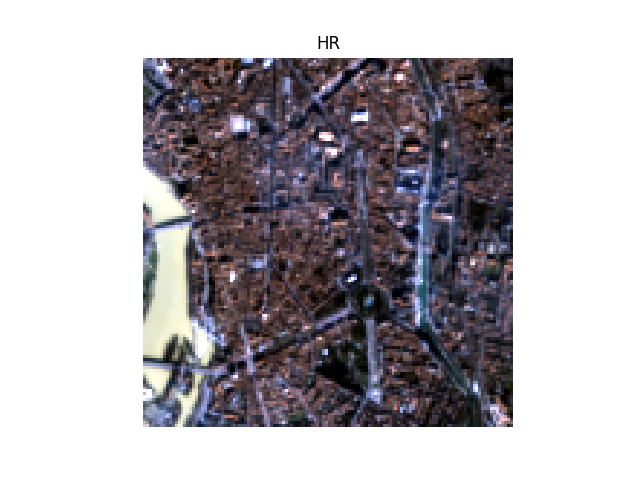
\includegraphics[scale=.5]{toulouse.png}
    \caption{Multispectral Toulouse image used for all the tests}
    \label{fig:toulouse}
\end{figure}

\begin{figure}
    \centering
    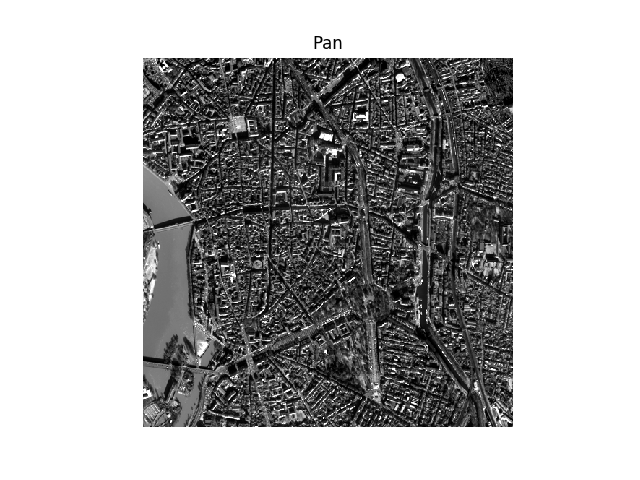
\includegraphics[scale=.5]{toulouse_pan.png}
    \caption{Pancromatic Toulouse image used for all the tests}
    \label{fig:toulouse_pan}
\end{figure}


All those type of training have been executed in a test image: the Fig. \ref{fig:toulouse} \ref{fig:toulouse_pan}.

\section{Results}
Using the original QNR function has not produce any positive results.
During the training, while the error continued to be minimized, the indices calculated with the Matlab Toolbox worsened as showed in Fig.~\ref{fig:qnr1}~\ref{fig:qnr2}~\ref{fig:qnr3}, even the QNR itself.
This because the algorithm, to minimize the error builded with the QNR developed in python, generate an image with negative values.
An input with negative values is not expected by any of the indexes used and this create a discrepancy between the QNR developed in python and the QNR of the Matlab Toolbox.
Indeed, the QNR developed in python and used in the loss function it was tested with regular images with values between 0 and 1 and it returned same results of the Matlab version.


\begin{figure}[t]
    \centering
    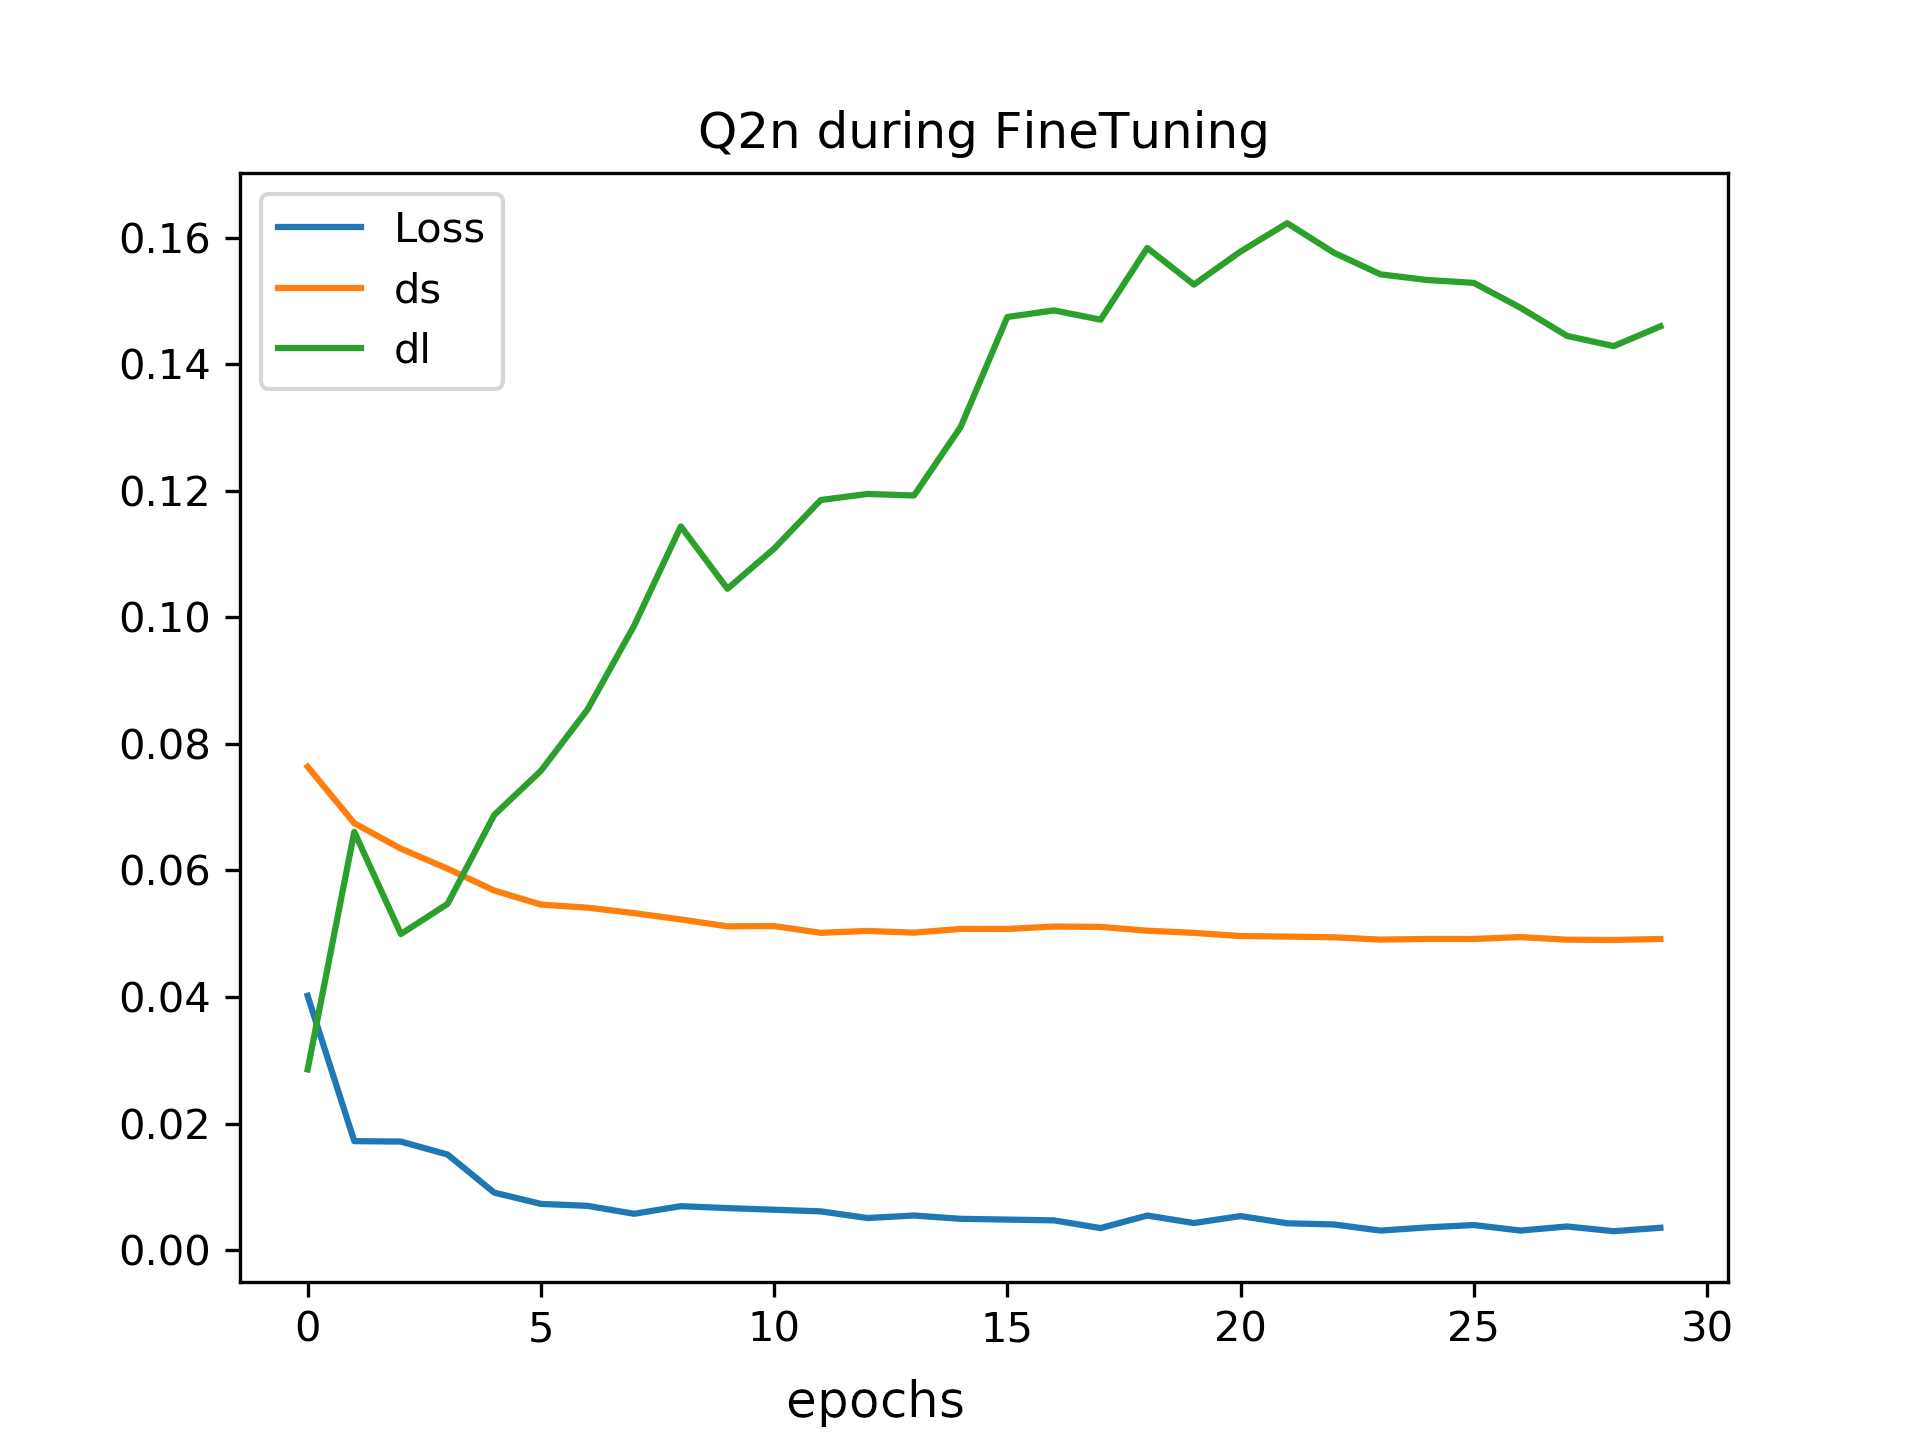
\includegraphics[scale=.5]{qnr1.png}
    \caption{Loss, DS and DL of QNR during the training}
    \label{fig:qnr1}
\end{figure}


\begin{figure}
    \centering
    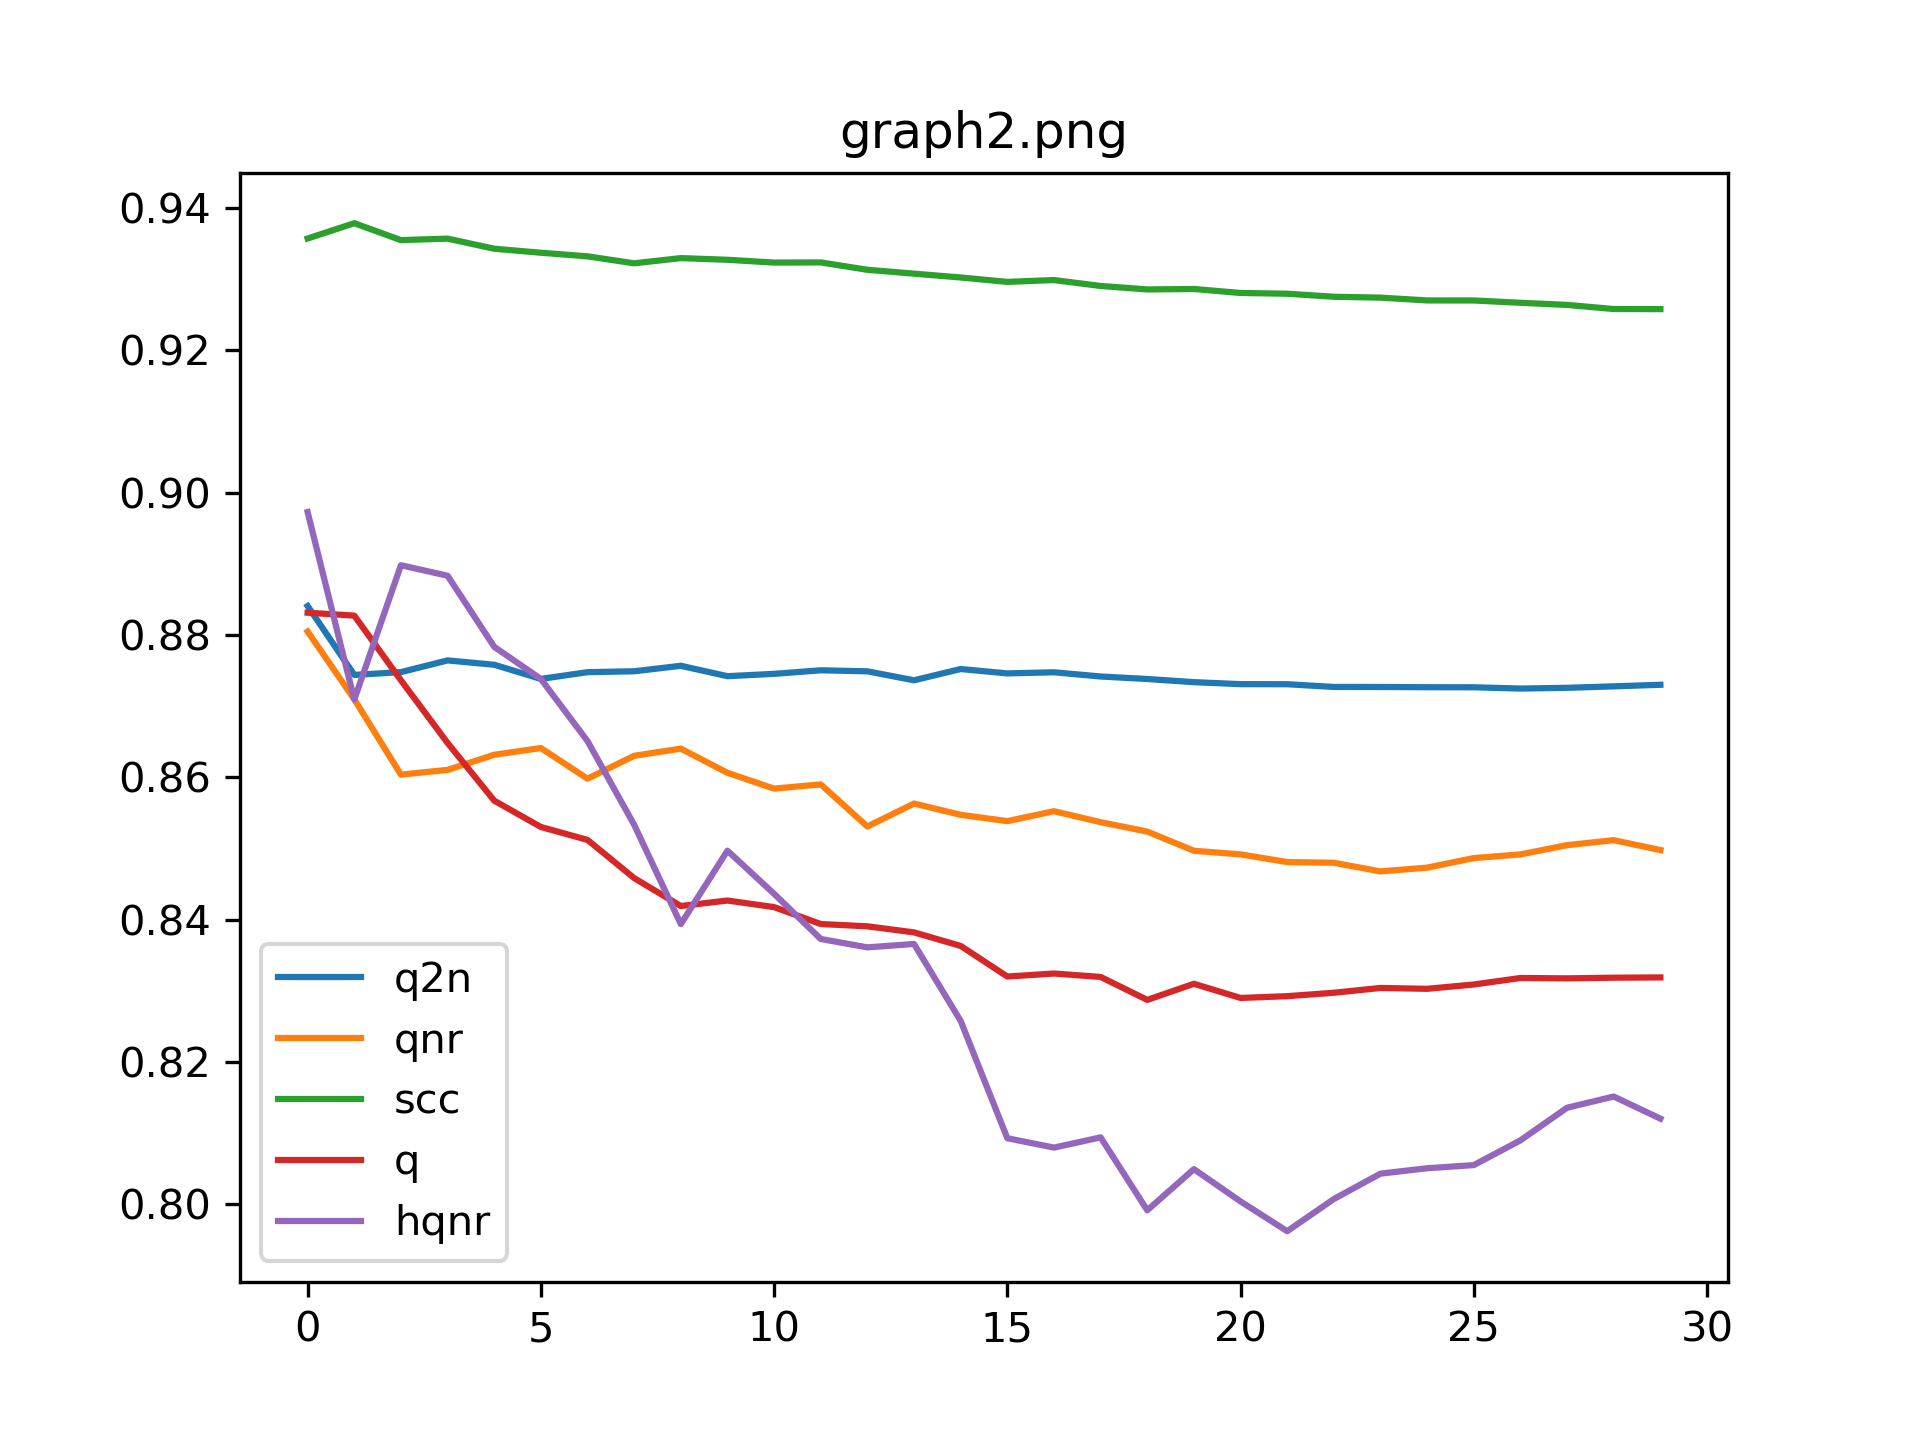
\includegraphics[scale=.5]{qnr2.png}
    \caption{Q2N, QNR, SCC, Q and HQNR during the training}
    \label{fig:qnr2}
\end{figure}


\begin{figure}
    \centering
    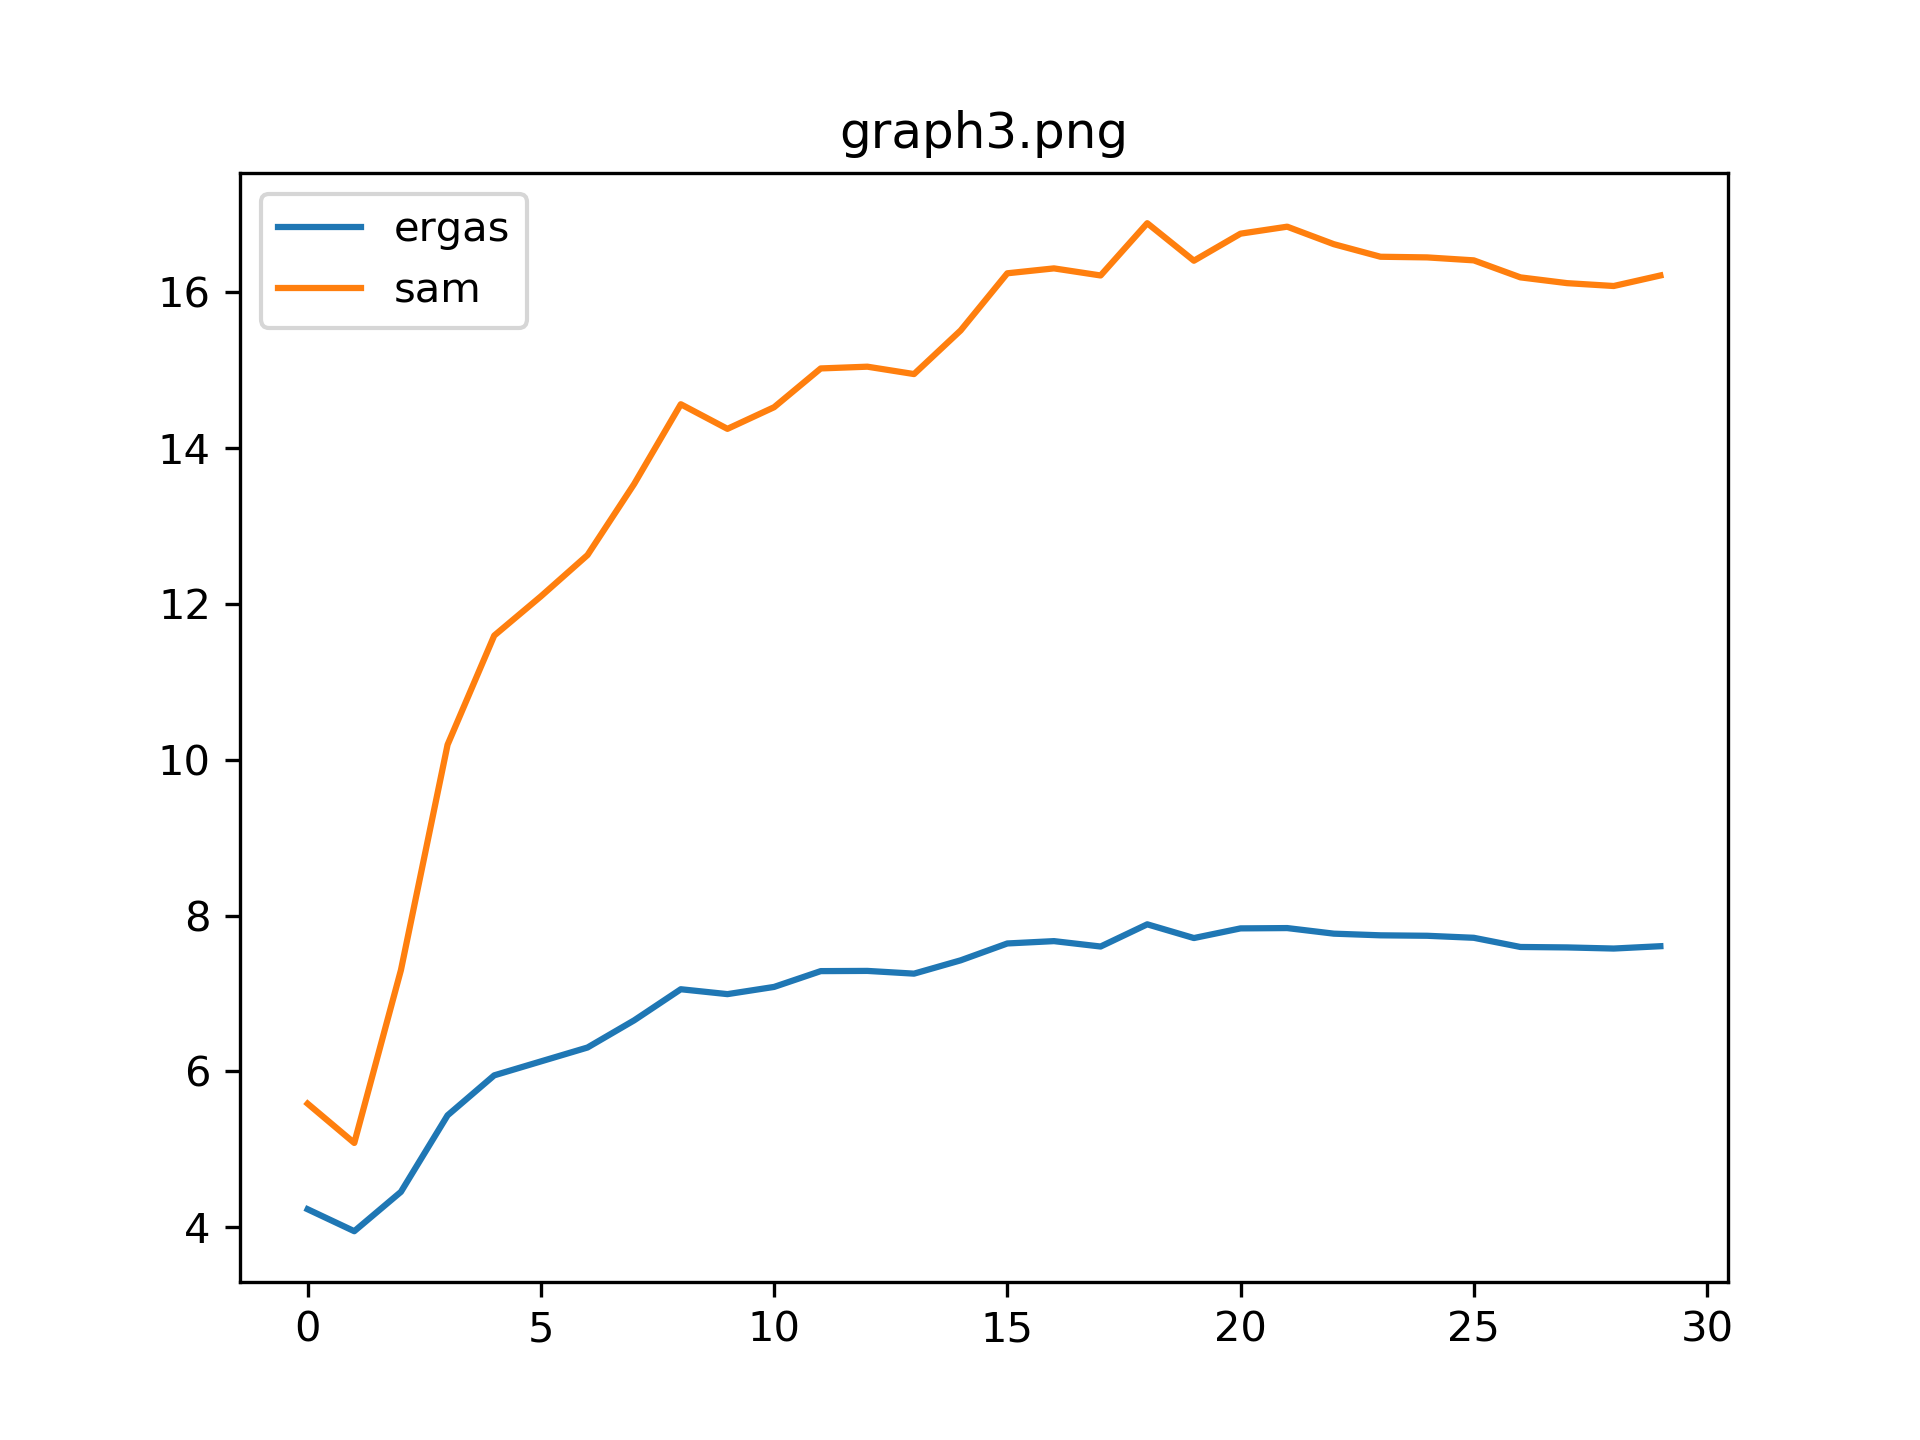
\includegraphics[scale=.5]{qnr3.png}
    \caption{ERGAS and SAM during the training}
    \label{fig:qnr3}
\end{figure}

The loss tends to reach his minimum value but this is not reflected in an increase of the quality indexes. 

After these tests, it was decided to change the loss function using another no-reference index: the HQNR.
But this index is more complex than the QNR because it involve quaternions and operations with hypercomplex numbers.

As described in the previous chapter, it was applied an approximated version of HQNR and in the following graphs (Fig.~\ref{fig:hqnr1})
the results are illustated for the Ikonos Toulouse image.


\begin{figure}[t]
    \centering
    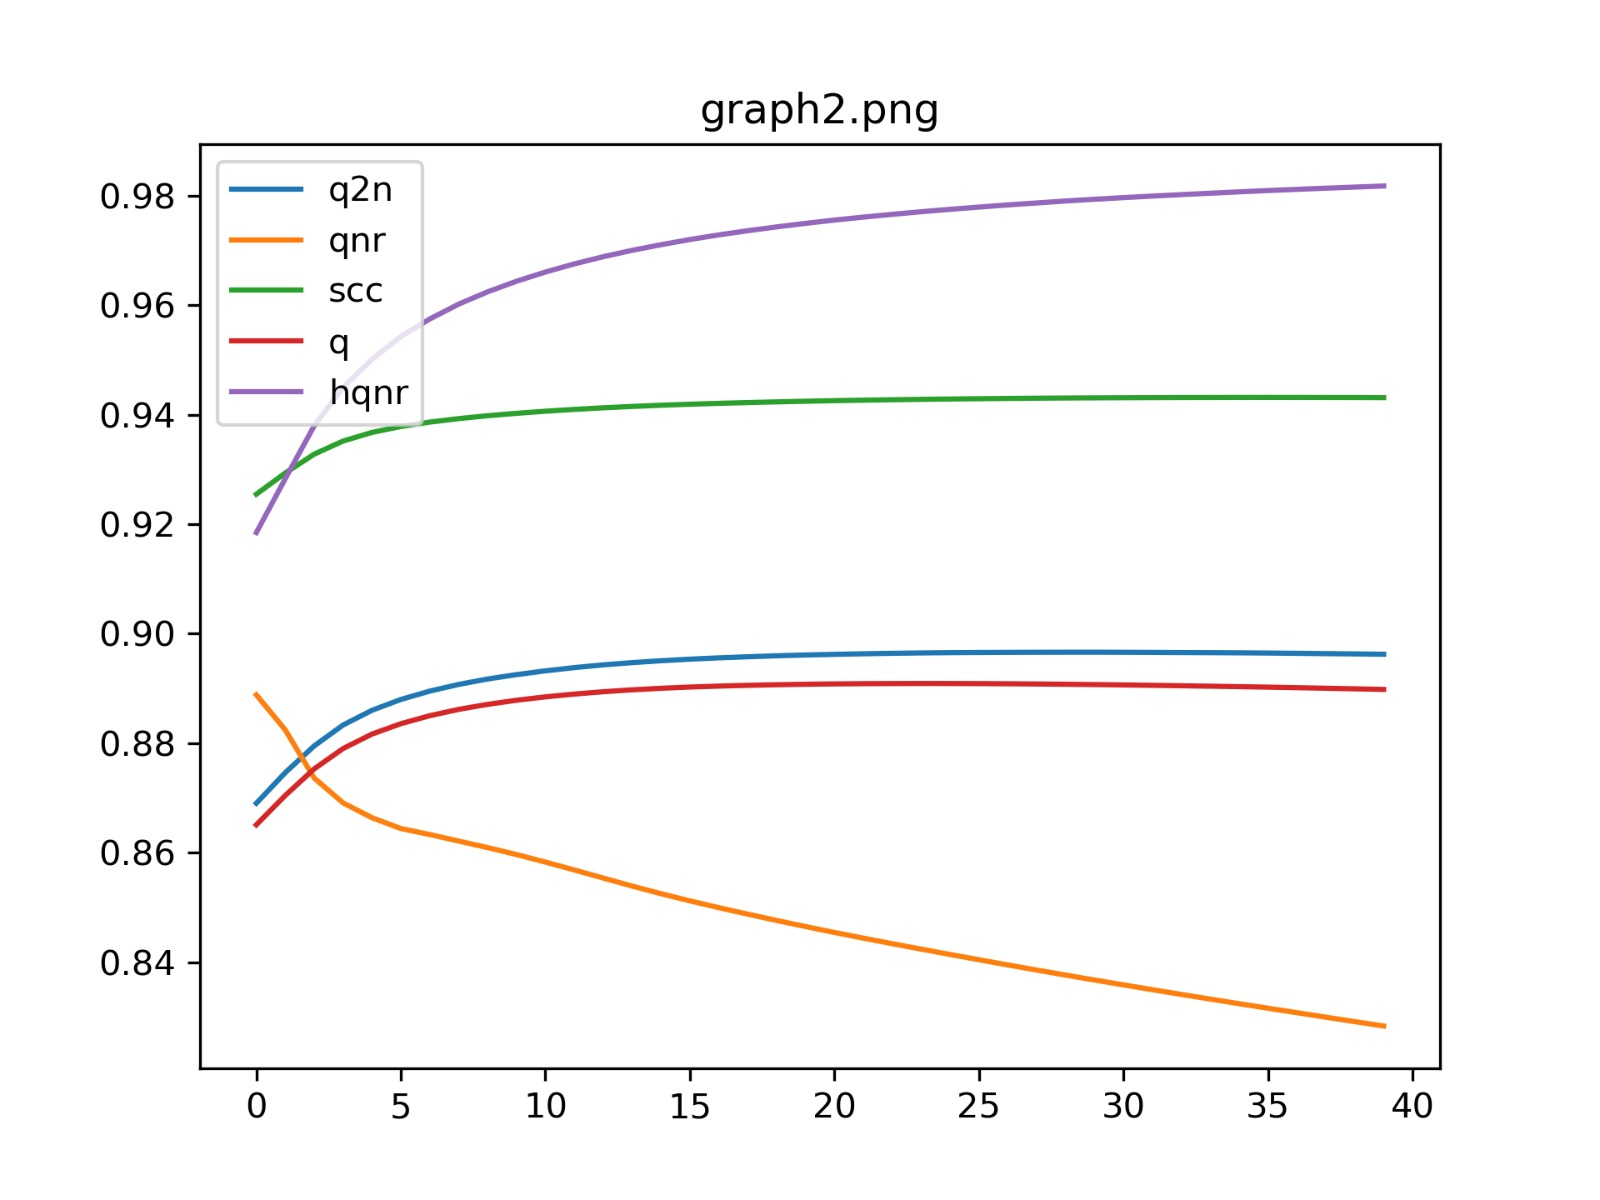
\includegraphics[scale=.2]{toulouse_noref.jpeg}
    \caption{Q2N, QNR, SCC, Q and HQNR during the training using the loss function with HQNR}
    \label{fig:hqnr1}
\end{figure}

With this type of loss function it was recorded an increase in all the indexes except for the QNR.
The QNR, as evidenced also by the previous results, does not seems to be a good index for the quality assessment.

To explore all the possible values of q and p in the Eq.~\ref{dl}~\ref{ds}, 
test with different values has been lauched. At the beginning with steps of 0.5 and after for particupar ranges with steps of 0.25.

In Fig. \ref{fig:alpha_beta1} and \ref{fig:alpha_beta3}, in the legend the first argument is alpha and the second is beta.
They are the inverse respectively of p and q. 

\begin{figure}[t]
    \centering
    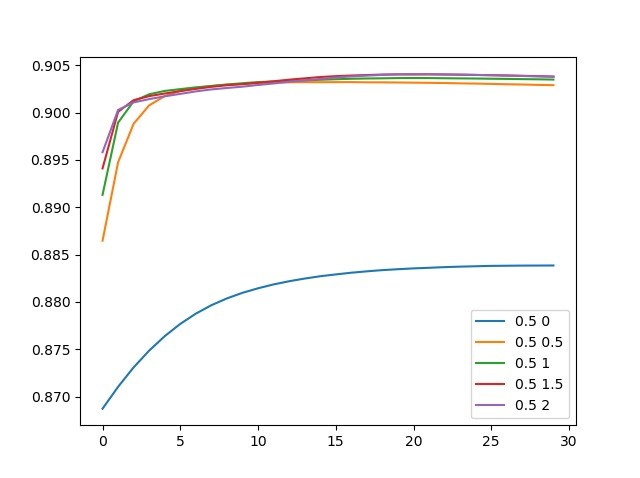
\includegraphics[scale=.5]{alpha_beta1.jpeg}
    \caption{Alpha and Beta with a 0.5 step}
    \label{fig:alpha_beta1}
\end{figure}


\begin{figure}
    \centering
    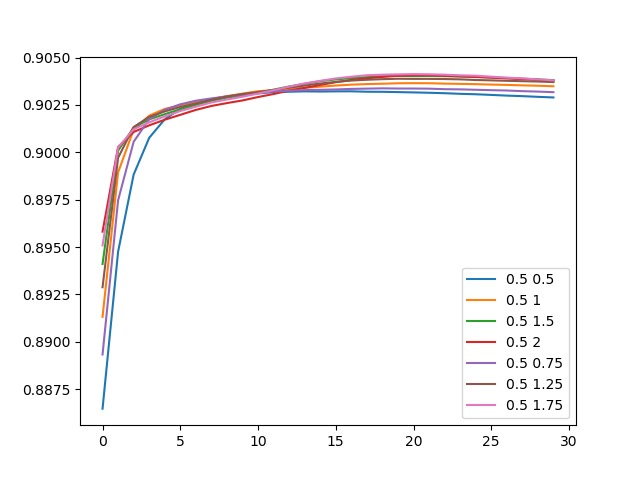
\includegraphics[scale=.5]{alpha_beta3.jpeg}
    \caption{Beta with a 0.25 step between beta 0.5 and beta 2 and alpha setted to 0.5}
    \label{fig:alpha_beta3}
\end{figure}

The experiment conclusion was that best result are reached with alpha 0.5 and beta 2.

\chapter*{Conclusions}
``I always thought something was fundamentally wrong with the universe'' \cite{criticalComparison}
\newpage

\bibliographystyle{unsrt}
\bibliography{references}

\newpage

\appendix

\begin{spacing}{1}
\section{QNR}
\label{qnr_functions}
\lstinputlisting[language=python]{qnr.py}

\section{HQNR}
\label{hqnr_functions}
\lstinputlisting[language=python]{hqnr.py}
\end{spacing}

\end{document}

